\RequirePackage[l2tabu,orthodox]{nag}

% TODO: decide if one-sided/two-sided
%\documentclass[headsepline,footsepline,footinclude=false,fontsize=11pt,paper=a4,listof=totoc,bibliography=totoc,BCOR=12mm,DIV=12]{scrbook} % two-sided
\documentclass[headsepline,footsepline,footinclude=false,oneside,fontsize=11pt,paper=a4,listof=totoc,bibliography=totoc]{scrbook} % one-sided

% TODO: change citation style in settings
\PassOptionsToPackage{table,svgnames,dvipsnames}{xcolor}


\usepackage{amsmath,amssymb,amsthm,graphicx,wrapfig,paralist}
\usepackage{algorithmicx,algorithm}
\usepackage[noend]{algpseudocode}
\usepackage{booktabs}
\usepackage{proof}
\usepackage{tikz}
\usepackage{graphics}
\usepackage{stmaryrd}
\usepackage{wasysym}

\usepackage{ellipsis, mparhack, ragged2e} % bugfixing
\usepackage[l2tabu, orthodox]{nag} % avoid typical LaTeX errors

\usepackage{tabu,multirow}
\usepackage{xparse}
\usepackage{mathtools}
\usepackage{environ}

\usepackage[ngerman,american]{babel}
% \usepackage[latin1]{inputenc}
% \usepackage[pdftex]{hyperref}

\usepackage{caption}
%\usepackage{subcaption}

\usepackage{algpseudocode}

\usepackage{marginfix}
\usepackage{xifthen}

\usepackage{scrhack} % necessary for listings package
\usepackage{listings}

%\usepackage{listings}
%\lstdefinestyle{customJ}{
%  belowcaptionskip=1\baselineskip,
% breaklines=true,
%  frame=L,
%  xleftmargin=\parindent,
%  language=Java,
%  showstringspaces=false,
%  basicstyle=\footnotesize\ttfamily,
%  keywordstyle=\bfseries\color{green!40!black},
%  commentstyle=\itshape\color{purple!40!black},
%  identifierstyle=\color{blue},
%  stringstyle=\color{orange},
%}

\usepackage{afterpage}
\newcommand\blankpage{%
    \null
    \thispagestyle{empty}%
    \newpage}

\renewcommand{\arraystretch}{1.2}


\usepackage[utf8]{inputenc}
\usepackage[T1]{fontenc}
\usepackage[sc]{mathpazo}
\usepackage[autostyle]{csquotes}
\usepackage[%
  backend=biber,
  url=false,
  style=alphabetic,
  maxnames=4,
  minnames=3,
  maxbibnames=99,
  giveninits,
  uniquename=init]{biblatex} % TODO: adapt citation style
%\addbibresource{bibliography.bib}
\usepackage{subfig}
\usepackage{todonotes}
\usepackage{scrhack} % necessary for listings package
\usepackage{listings}
\usepackage{lstautogobble}
\usepackage{pgfplots}
\usepackage{pgfplotstable}
\usepackage[final]{microtype}
\usepackage[hidelinks]{hyperref} % hidelinks removes colored boxes around references and links

\bibliography{bibliography}

\setkomafont{disposition}{\normalfont\bfseries} % use serif font for headings
\linespread{1.05} % adjust line spread for mathpazo font

% Add table of contents to PDF bookmarks
\BeforeTOCHead[toc]{{\cleardoublepage\pdfbookmark[0]{\contentsname}{toc}}}

% Define TUM corporate design colors
% Taken from http://portal.mytum.de/corporatedesign/index_print/vorlagen/index_farben
\definecolor{TUMBlue}{HTML}{0065BD}
\definecolor{TUMSecondaryBlue}{HTML}{005293}
\definecolor{TUMSecondaryBlue2}{HTML}{003359}
\definecolor{TUMBlack}{HTML}{000000}
\definecolor{TUMWhite}{HTML}{FFFFFF}
\definecolor{TUMDarkGray}{HTML}{333333}
\definecolor{TUMGray}{HTML}{808080}
\definecolor{TUMLightGray}{HTML}{CCCCC6}
\definecolor{TUMAccentGray}{HTML}{DAD7CB}
\definecolor{TUMAccentOrange}{HTML}{E37222}
\definecolor{TUMAccentGreen}{HTML}{A2AD00}
\definecolor{TUMAccentLightBlue}{HTML}{98C6EA}
\definecolor{TUMAccentBlue}{HTML}{64A0C8}

% Settings for pgfplots
\pgfplotsset{compat=newest}
\pgfplotsset{
  % For available color names, see http://www.latextemplates.com/svgnames-colors
  cycle list={TUMBlue\\TUMAccentOrange\\TUMAccentGreen\\TUMSecondaryBlue2\\TUMDarkGray\\},
}

% Settings for lstlistings
\lstset{%
  basicstyle=\ttfamily,
  columns=fullflexible,
  autogobble,
  keywordstyle=\bfseries\color{TUMBlue},
  stringstyle=\color{TUMAccentGreen}
}

\usepackage[acronym,xindy,toc]{glossaries} % TODO: include "acronym" if glossary and acronym should be separated
\makeglossaries
\loadglsentries{pages/glossary.tex}

%%\usepackage[bookmarks]{hyperref}
\usepackage{amsmath,amssymb,xcolor,graphicx,wrapfig,paralist}
\usepackage{algorithmicx,algorithm}
\usepackage[noend]{algpseudocode}
\usepackage{booktabs}
\usepackage{proof}
\usepackage{tikz}
\usepackage{csquotes}
\usepackage{graphics}
\usepackage{stmaryrd}
%\usepackage[caption=false]{subfig}

\usepackage{ellipsis, mparhack, ragged2e} % bugfixing
\usepackage[l2tabu, orthodox]{nag} % avoid typical LaTeX errors

\usepackage{tabu,multirow}
\usepackage{xparse}
\usepackage{mathtools}
\usepackage{environ}

%\usepackage[english]{babel}
% \usepackage[latin1]{inputenc}
% \usepackage[pdftex]{hyperref}

\usepackage{caption}
%\usepackage{subcaption}

\usepackage{algorithm}
\usepackage{algpseudocode}

\usepackage{marginfix}
\usepackage{xifthen}

\usepackage{listings}
\lstdefinestyle{customJ}{
  belowcaptionskip=1\baselineskip,
  breaklines=true,
  frame=L,
  xleftmargin=\parindent,
  language=Java,
  showstringspaces=false,
  basicstyle=\footnotesize\ttfamily,
  keywordstyle=\bfseries\color{green!40!black},
  commentstyle=\itshape\color{purple!40!black},
  identifierstyle=\color{blue},
  stringstyle=\color{orange},
}

\usepackage{afterpage}
%\newcommand\blankpage{%
%    \null
%    \thispagestyle{empty}%
%    \newpage}

\renewcommand{\arraystretch}{1.2}



%\newcommand{\gls}[1]{#1}
% == TODOs
\newcommand{\highlight}[1]{\textsf{\textbf{#1}}}
\newcommand{\todojan}[1]{\todo{\textbf{Ja:\\}#1}}
\newcommand{\todojulia}[1]{\todo{\highlight{Ju:\\}#1}}
\newcommand{\fix}[2][\relax]{\marginpar{{\footnotesize \textbf{#1}\par #2}}}

% == ALGORITHMS
\renewcommand{\algorithmicrequire}{\textbf{Input:}}
\renewcommand{\algorithmicensure}{\textbf{Output:}}
\algrenewcommand{\algorithmiccomment}[1]{\hskip1.5em \textbackslash *  #1 * \textbackslash}

% == TABLES
\newcolumntype{L}{X}
\newcolumntype{R}{>{\raggedleft\arraybackslash}X}
\newcolumntype{C}{>{\centering\arraybackslash}X}

% == GRAPHICS
\DeclareGraphicsExtensions{.pdf, .png, .jpg}

% == LATEX
\newcommand\numberthis{\addtocounter{equation}{1}\tag{\theequation}}

% == THEOREMS
\newtheorem{theorem}{Theorem}[section]
\newtheorem{corollary}{Corollary}[theorem]
\newtheorem{lemma}[theorem]{Lemma}
\newtheorem{definition}{Definition}[section]


% == SPACE

%\usepackage{microtype}
%\renewcommand{\baselinestretch}{0.975} % >=0.97

%\newcommand{\spacefu}{\vspace*{-1.2em}}
%\newcommand{\spacefl}{\vspace*{-0.8em}}
%\newcommand{\myspace}{\vspace*{-0.5em}}

% == TODO

%\NewDocumentCommand{\todo}{m}{%
%	% Add to todo list
%	\begin{tikzpicture}[remember picture, baseline=-0.75ex]%
%	\node [coordinate] (inText) {};%
%	\end{tikzpicture}%
%	%
%	% Make the margin par
%	\marginpar{%
%		\begin{tikzpicture}[remember picture, font=\scriptsize]%
%		\draw node[draw=red, text width = 3.5cm, inner sep=0.3mm] (inNote){#1};%
%		\end{tikzpicture}%
%	}%
%	\begin{tikzpicture}[remember picture, overlay]%
%	\draw[draw=red]%
%	([yshift=-0.2cm] inText)%
%	% -| ([xshift=-0.05cm] inNote.west)%
%	-| (inNote.south);%
%	\end{tikzpicture}%
%}%

% == SYMBOLS

\RequirePackage{marvosym}
\providecommand{\contradiction}{\Lightning}


% == BOOLEAN

\newcommand{\boolor}{\vee}
\newcommand{\booland}{\wedge}
\newcommand{\boolOr}{\bigvee}
\newcommand{\boolAnd}{\bigwedge}
\newcommand{\boolnot}{\lnot}


% == BASIC OPERATORS

\DeclarePairedDelimiter{\delimabs}{\lvert}{\rvert}
\DeclarePairedDelimiter{\delimnorm}{\lVert}{\rVert}
\DeclarePairedDelimiter{\delimpospart}{\lgroup}{\rgroup^+}
\DeclarePairedDelimiter{\delimnegpart}{\lgroup}{\rgroup^-}
\DeclarePairedDelimiterX{\deliminner}[2]{\lange}{\rangle}{#1, #2}
\DeclarePairedDelimiter{\delimcardinality}{\lvert}{\rvert}
\DeclarePairedDelimiter{\delimset}{\lbrace}{\rbrace}
\DeclarePairedDelimiter{\delimtuple}{(}{)}
\DeclarePairedDelimiter{\delimlistt}{[}{]}
\DeclarePairedDelimiter{\delimfun}{(}{)}

\NewDocumentCommand{\abs}{sm}{\IfBooleanTF{#1}{\delimabs{#2}}{\delimabs*{#2}}}
\NewDocumentCommand{\norm}{sm}{\IfBooleanTF{#1}{\delimnorm{#2}}{\delimnorm*{#2}}}
\NewDocumentCommand{\pospart}{sm}{\IfBooleanTF{#1}{\delimpospart{#2}}{\delimpospart*{#2}}}
\NewDocumentCommand{\negpart}{sm}{\IfBooleanTF{#1}{\delimnetpart{#2}}{\delimnetpart*{#2}}}
\NewDocumentCommand{\inner}{sm}{\IfBooleanTF{#1}{\deliminner{#2}}{\deliminner*{#2}}}
\NewDocumentCommand{\cardinality}{sm}{\IfBooleanTF{#1}{\delimcardinality{#2}}{\delimcardinality*{#2}}}
\NewDocumentCommand{\set}{sm}{\IfBooleanTF{#1}{\delimset*{#2}}{\delimset{#2}}}
\NewDocumentCommand{\tuple}{sm}{\IfBooleanTF{#1}{\delimtuple{#2}}{\delimtuple*{#2}}}
\NewDocumentCommand{\closure}{sm}{\IfBooleanTF{#1}{\delimclosure{#2}}{\delimclosure*{#2}}}
\NewDocumentCommand{\listt}{sm}{\IfBooleanTF{#1}{\delimlistt{#2}}{\delimlistt*{#2}}}
\NewDocumentCommand{\fun}{smm}{\IfBooleanTF{#1}{{#2}\delimfun{#3}}{{#2}\delimfun*{#3}}}
\NewDocumentCommand{\funMacro}{smm}{\IfNoValueTF{#3}{#1}{\fun{#2}{#3}}}

\DeclareMathOperator{\ExistsOp}{\exists}
\DeclareMathOperator{\ForallOp}{\forall}

\NewDocumentCommand{\Exists}{gg}{\IfNoValueTF{#1}{\ExistsOp}{\ExistsOp #1. \, #2}}
\NewDocumentCommand{\Forall}{gg}{\IfNoValueTF{#1}{\ForallOp}{\ForallOp #1. \, #2}}

\DeclarePairedDelimiter\ceil{\lceil}{\rceil}
\DeclarePairedDelimiter\floor{\lfloor}{\rfloor}


% == SETS OPERATORS

\newcommand{\setcomplement}[1]{{#1}^c}
\newcommand{\powerset}[1]{\mathcal{P}(#1)}

\newcommand{\unionSym}{\cup}
\newcommand{\unionBin}{\mathbin{\unionSym}}
\newcommand{\strictunionSym}{\dot{\unionSym}}
\newcommand{\strictunionBin}{\mathbin{\dot{\unionSym}}}
\newcommand{\intersectionSym}{\cap}
\newcommand{\intersectionBin}{\mathbin{\intersectionSym}}
\newcommand{\UnionSym}{\bigcup}
\newcommand{\UnionBin}{\mathbin{\UnionSym}}
\newcommand{\strictUnionSym}{\dot{\UnionSym}}
\newcommand{\strictUnionBin}{\mathbin{\strictUnionSym}}
\newcommand{\IntersectionSym}{\bigcap}
\newcommand{\IntersectionBin}{\mathbin{\IntersectionSym}}

\newcommand{\union}{\unionBin}
\newcommand{\strictunion}{\strictunionBin}
\newcommand{\intersection}{\intersectionBin}
\newcommand{\Union}{\UnionSym}
\newcommand{\strictUnion}{\strictUnionSym}
\newcommand{\Intersection}{\IntersectionSym}


% == BASIC SETS

\newcommand{\Continuous}{C}
\newcommand{\Sobolev}{\mathcal{W}}
\newcommand{\Naturals}{\mathbb{N}}
\newcommand{\Domain}{\mathfrak{D}}
\newcommand{\Measures}{\mathcal{M}}
\newcommand{\Lebesgue}{\mathcal{L}}
\newcommand{\Hilb}{H}
\newcommand{\Reals}{\mathbb{R}}
\newcommand{\Orlicz}{{\tilde{\Lebesgue}}}
\newcommand{\Distributions}{\mathcal{D}}


% == LIMITS

\NewDocumentCommand{\convto}{G{}}{\xrightarrow{#1}}
\NewDocumentCommand{\weakto}{G{}}{\xrightharpoonup{#1}}
\NewDocumentCommand{\weakstarto}{G{}}{\xrightharpoonup[*]{#1}}

% == OPERATORS

\newcommand{\gradient}{\nabla}
\newcommand{\laplacian}{\Delta}
 \DeclareDocumentCommand{\diff}{D<>{} O{}  D(){}}{\Delta_{#1}^{#2}\ifthenelse{\isempty{#3}}{}{(#3)}}
\newcommand{\boundary}{\partial}
\DeclareMathOperator{\divergence}{div}
\DeclareMathOperator{\distance}{dist}
\DeclareMathOperator{\esssup}{ess sup}
\DeclareMathOperator{\supp}{supp}
\DeclareMathOperator{\capacity}{cap}
\DeclareMathOperator{\signum}{signum}
\DeclareMathOperator{\id}{id}
\DeclareMathOperator{\const}{const}
\DeclareMathOperator{\loc}{loc}
\DeclareMathOperator*{\argmax}{arg\, max}
\DeclareMathOperator*{\argmin}{arg\, min}
\DeclareDocumentCommand{\post}{D<>{} O{} D(){}}{\mathsf{Post}_{#1}^{#2}\ifthenelse{\isempty{#3}}{}{(#3)}}
\DeclareMathOperator{\leaves}{\mathsf{leaves}}
\DeclareMathOperator{\stays}{\mathsf{stays\_in}}
\newcommand{\eqdef}{\vcentcolon=}
\newcommand{\defeq}{=\vcentcolon}

\newcommand{\qee}{\hfill$\triangle$} % quod erat exemplandum % TODO del

% == LOGIC

\newcommand{\ltl}{\operatorname{LTL}}
\newcommand{\ctl}{\operatorname{CTL}}
\newcommand{\pctl}{\operatorname{pCTL}}
\newcommand{\Next}{\varbigcirc}
\newcommand{\until}{\, \mathcal{U}}
\newcommand{\wrel}{\mathcal{W}}
\newcommand{\lang}[1]{\mathcal{L}(#1)}
\newcommand{\reach}{\Diamond}
\newcommand{\alws}{\Box}
\newcommand{\true}{\mathsf{true}}
\newcommand{\false}{\mathsf{false}}
\newcommand{\turn}{\mathsf{turn}}
\newcommand{\PQ}{\mathrm{PQ}}

% == COMPLEXITY
\newcommand{\NP}{\mathbf{NP}}
\newcommand{\NEXP}{\mathbf{NEXP}}
\newcommand{\PSPACE}{\mathbf{PSPACE}}

% == PROBABILITY
\NewDocumentCommand{\distributions}{d()}{\funMacro{\mathcal{D}}{#1}}
\newcommand{\dirac}[1]{\delta_{#1}}
\newcommand{\probability}{\mathbb{P}}
\newcommand{\expectation}{\mathbb{E}}

% == MC, MPD, Games

\newcommand{\gain}{g} %value
\newcommand{\bias}{b}
\newcommand{\stat}{q}
\newcommand{\outcomes}{\mathcal{O}}
\newcommand{\salgebra}{\mathcal{F}}
\newcommand{\mevent}{\mathcal{E}}
\newcommand{\pmin}{p_{\min}}
\newcommand{\rmax}{r_{\max}}
\newcommand{\MECs}{\mathsf{MEC}}
\newcommand{\GCs}{\mathsf{GC}}
\DeclareDocumentCommand{\val}{D<>{} O{}  D(){} t'}{\mathsf{V}_{#1}^{\IfBooleanTF{#4}{\prime #2}{#2}}\ifthenelse{\isempty{#3}}{}{(#3)}}
\DeclareDocumentCommand{\game}{D<>{} O{} D(){} t'}{\mathsf{G}_{#1}^{\IfBooleanTF{#4}{\prime}{}#2}\ifthenelse{\isempty{#3}}{}{(#3)}}
\DeclareDocumentCommand{\transition}{D<>{} O{} D(){}}{\rightarrow_{#1}^{#2}\ifthenelse{\isempty{#3}}{}{(#3)}}


\newcommand{\Ts}{\mathcal{T}}
\newcommand{\Mc}{\mathsf{M}}
\newcommand{\Mdp}{\mathcal{M}}
\newcommand{\Pm}{\mathbf{P}}
\newcommand{\SG}{\textrm{SG}}
\newcommand{\SGs}{\textrm{SGs}}
\DeclareDocumentCommand{\G}{D<>{} O{} t' D(){}}{\mathsf{G}_{#1}^{\IfBooleanTF{#3}{\prime}{}#2}\ifthenelse{\isempty{#4}}{}{(#4)}}
\DeclareDocumentCommand{\exGame}{D<>{} O{} t'  D(){}}{\mathsf{G}_{#1}^{\IfBooleanTF{#3}{\prime}{}#2}\ifthenelse{\isempty{#4}}{}{(#4)}=(\states<#1>[\IfBooleanTF{#3}{\prime}{}#2],\states<\Box\ifthenelse{\isempty{#1}}{}{,#1}>[\IfBooleanTF{#3}{\prime}{}#2],\states<\circ\ifthenelse{\isempty{#1}}{}{,#1}>[\IfBooleanTF{#3}{\prime}{}#2],\istate<#1>[\IfBooleanTF{#3}{\prime}{}#2],\actions<#1>[\IfBooleanTF{#3}{\prime}{}#2],\Av<#1>[\IfBooleanTF{#3}{\prime}{}#2],\trans<#1>[\IfBooleanTF{#3}{\prime}{}#2])}


\newcommand{\ap}{Ap}
\newcommand{\states}{\mathsf{S}}
\DeclareDocumentCommand{\state}{D<>{} O{}  t'}{\mathsf{s}_{#1}^{\IfBooleanTF{#3}{\prime #2}{#2}}}
\DeclareDocumentCommand{\istate}{D<>{} O{} t'}{\mathsf{s}_{0\ifthenelse{\isempty{#1}}{}{,#1}}^{\IfBooleanTF{#3}{\prime~#2}{#2}}}
\newcommand{\inv}{\nu}
\newcommand{\lab}{L}

\newcommand{\edges}{E}
\newcommand{\statesone}{S^N}
\newcommand{\statestwo}{S_2}
\newcommand{\statesp}{S^P}
\newcommand{\initstate}{\state<0>}
\newcommand{\initdist}{\mu}
\DeclareDocumentCommand{\trans}{D<>{} O{} t' D(){} D(){}}{\delta_{#1}^{\IfBooleanTF{#3}{\prime}{}#2}\ifthenelse{\isempty{#4}}{}{(#4)}\ifthenelse{\isempty{#5}}{}{(#5)}}
\DeclareDocumentCommand{\Av}{D<>{} O{} t' D(){}}{\mathsf{Av}_{#1}^{\IfBooleanTF{#3}{\prime}{}#2}\ifthenelse{\isempty{#4}}{}{(#4)}}
\newcommand{\rew}{r}
\DeclareDocumentCommand{\F}{D<>{} O{} t' D(){}}{\mathsf{F}_{#1}^{\IfBooleanTF{#3}{\prime}{}#2}\ifthenelse{\isempty{#4}}{}{(#4)}}
\newcommand{\lu}{\hat{l},\hat{u}}

% = paths and strategies
\newcommand{\Path}{\rho}
\DeclareDocumentCommand{\Path}{D<>{} O{} t' D(){}}{\path<#1>[#2]\IfBooleanTF{#3}{'}{}(#4)}
\DeclareDocumentCommand{\path}{D<>{} O{} t' D(){}}{\rho_{#1}^{\IfBooleanTF{#3}{\prime}{}#2}\ifthenelse{\isempty{#4}}{}{(#4)}}
\newcommand{\fpath}{\mathsf{w}}
\DeclareDocumentCommand{\Paths}{D<>{} O{} t' D(){}}{\Omega_{#1}^{\IfBooleanTF{#3}{\prime}{}#2}\ifthenelse{\isempty{#4}}{}{(#4)}}
\newcommand{\straa}{\sigma}
\newcommand{\straas}{\Sigma}
\newcommand{\strab}{\tau}
\newcommand{\strabs}{\Tau}
\newcommand{\plays}{\mathsf{Plays}}
\newcommand{\play}{\mathsf{Play}}
\newcommand{\last}[1]{#1\mathord\downarrow}
\DeclareDocumentCommand{\strategy}{D<>{} O{} D(){}
  t*}{{\IfBooleanTF{#4}{\tau}{\sigma}}_{#1}^{#2}\ifthenelse{\isempty{#3}}{}{(#3)}}

% = probability

\newcommand{\inits}{\hat s}
\DeclareDocumentCommand{\actions}{D<>{} O{} t' d()}{{\IfNoValueTF{#4}{\mathsf{A}}{\fun{\mathsf{A}}{#4}}}_{#1}^{\IfBooleanTF{#3}{\prime~#2}{#2}}}
\DeclareDocumentCommand{\action}{D<>{} O{} t'}{\mathsf{a}_{#1}^{\IfBooleanTF{#3}{\prime#2}{#2}}}
\newcommand{\pat}{\omega}
\newcommand{\Pat}{\mathsf{Runs}}
\newcommand{\fpat}{w}
\newcommand{\mem}{\mathsf{M}}
\newcommand{\Cone}{\mathsf{Cone}}
\newcommand{\calF}{\mathcal{F}}
\newcommand{\mec}{\mathsf{MEC}}
\newcommand{\scc}{\mathsf{SCC}}
\newcommand{\ec} {\mathsf{EC}}
\newcommand{\bscc}{\mathsf{BSCC}}

\newcommand{\attractor}{\mathsf{prob1}}
\newcommand{\pr}{\mathbb P}
\renewcommand{\Pr}[3]{\pr^{#1}\hspace{-0.16em}\left[{#3}\right]}   %\Pr{strat}{state}{event}
\newcommand{\PrS}[3]{\pr^{#1}_{#2}\hspace{-0.16em}\left[{#3}\right]}   %\Pr{strat}{state}{event}
\newcommand{\expected}{\mathbb{E}}
\newcommand{\expsucc}{\expected_\trans}
\newcommand{\Ex}[3]{\expected^{#1}_{#2}\hspace{-0.16em}\left[{#3}\right]}   %\Ex{strat}{state}{f}
\newcommand{\ExS}[3]{\expected^{#1}_{#2}\hspace{-0.16em}\left[{#3}\right]}   %\Ex{strat}{state}{f}


% == LOCAL

\newcommand{\push}{\mathrm{push}}
\newcommand{\pop}{\mathrm{pop}}
\newcommand{\topx}{\mathrm{top}}


\newcommand{\reward}{\vec{r}}
\newcommand{\ex}{\vecl{exp}}
\newcommand{\sat}{\vecl{sat}}
\newcommand{\satscalar}{\mathit{sat}}
\newcommand{\psat}{\vecl{pr}}%{\vec{p^{sat}}}
\newcommand{\psatscalar}{\mathit{pr}}%{\mathit{p^{sat}}}

\newcommand{\lrLim}[1]{\mathrm{lr}(#1)}  %\lr{rew}{run}
\newcommand{\lrSf}[1]{\mathrm{lr}_{\mathrm{sup}}(#1)}  %\lrS{rew}{run}
\newcommand{\lrIf}[1]{\mathrm{lr}_{\mathrm{inf}}(#1)}  %\lrI{rew}{run}
\newcommand{\lrInf}{\mathrm{lr}^{\mathrm{inf}}}  %\lrI{rew}{run}

\newcommand{\appear}{\textsf{Appear}}

\NewDocumentCommand{\spannorm}{m}{\fun{\operatorname{sp}}{#1}}

% == OTHER
\newcommand{\best}{\mathsf{best}}
\newcommand{\ebest}{\epsilon\textit{-}\mathsf{best}}
\newcommand{\Vis}{\mathsf{Vis}}
\DeclareDocumentCommand{\target}{D<>{} O{}
  t'}{\mathsf{f}_{#1}^{\IfBooleanTF{#3}{\prime}{}#2}}
\DeclareDocumentCommand{\fail}{D<>{} O{} t'}{\mathsf{\bot}_{#1}^{\IfBooleanTF{#3}{\prime}{}#2}}
\newcommand{\EXPLORE}{\mathsf{EXPLORE}}
\newcommand{\EXPLOREBREAK}{\mathsf{EXPLOREBREAK}}
\newcommand{\UPDATE}{\mathsf{UPDATE}}
\newcommand{\ADJUST}{\mathsf{ADJUST}}
\newcommand{\GETSUCC}{\mathsf{GETSUCC}}
\DeclareDocumentCommand{\CEC}{D<>{} O{} D(){}
  t*}{\IfBooleanTF{#4}{\simple~}{}\ifthenelse{\isempty{#3}}{}{#3\textit{-}}\textrm{CEC}_{#1}^{#2}}
\newcommand{\CCEC}{\circ\textit{-}\CEC}
\newcommand{\BCEC}{\Box\textit{-}\CEC}
\newcommand{\COLLAPSEFUN}{\mathsf{COLLAPSE\_SIMPLE}}
\newcommand{\COLLAPSEALG}{\mathsf{COLLAPSE}}
\newcommand{\simple}{\textit{simple}}
\newcommand{\Simple}{Simple}
\newcommand{\complex}{complex}
\newcommand{\Complex}{Complex}
\newcommand{\Succ}{\mathsf{Succ}}
\NewDocumentCommand{\exit}{D<>{}D[]{}D(){}}{\mathsf{bestExit}_{#1}^{#2}\ifthenelse{\isempty{#3}}{}{(#3)}}
\newcommand{\wexit}{\mathsf{worstExit}}
\newcommand{\reachSet}{\mathsf{reachSet}}
\newcommand{\creachSet}{\mathsf{compute\_reachSet}}
\newcommand{\cSucc}{\mathsf{compute\_Succ}}
\newcommand{\fsimBCEC}{\mathsf{Find\_\simple\_\BCEC{s}}}
\newcommand{\fstates}{\mathit{F}}
\newcommand{\rST}{\mathsf{runSampleTrial}}
\newcommand{\rSTA}{\mathsf{runSampleTrial_A}}
\newcommand{\BRTDPA}{\mathsf{BRTDP_A}}
\newcommand{\BRTDPC}{\mathsf{BRTDP_C}}

\newcommand{\chapterSpace}{\vspace*{1cm}}

% == Tikz
\newcommand{\drawcirc}{\node[draw,circle,minimum size=1.5cm]}
\newcommand{\drawbox}{\node[draw,rectangle,minimum size=1.5cm]}
\newcommand{\drawdummy}{\node[minimum size=0,inner sep=0]}



%%% Local Variables:
%%% mode: latex
%%% TeX-master: "../paper"
%%% End:
%SGs
\newcommand{\stateMac}{\mathsf{s}}
\newcommand{\valstra}{\mathsf{\val}_{\straa ,\strab}}
\newcommand{\valSolo}{\mathsf{\val}}
\newcommand{\reachProb}{p_{s}^{\straa, \strab}} %this could probably also be a big delta
\newcommand{\zeroSinks}{\mathit{Z}}
\newcommand{\zeroSink}{\mathrm{z}}
\newcommand{\sinks}{\zeroSinks}
\newcommand{\minStates}{\states_{\Circ}}
\newcommand{\maxStates}{\states_{\Box}}
\newcommand{\twoSucc}{\mathrm{\textbf{2Act}}}
\newcommand{\twoTrans}{\mathrm{\textbf{2Trans}}}
\newcommand{\halfProbss}{\mathrm{\textbf{2Trans}}}
\newcommand{\halfProbs}{\mathrm{\pmb{\frac{1}{2}}\textbf{Probs}}}
\newcommand{\stopping}{\mathrm{\textbf{Stopping game}}}
\newcommand{\noOneSucc}{\mathrm{\textbf{No1Act}}}
\newcommand{\s}{\state}
\newcommand{\cnf}{Condon's normal form}
\newcommand{\conQP}{Condon's quadratic program}
\newcommand{\actionb}{\mathsf{b}}
\newcommand{\valSum}{\sum\limits_{\mathsf{s_i} \in \post(\state, \action)} \trans(\state, \action, \mathsf{s_i}) \cdot \val(\mathsf{s_i})}

\newcommand{\Circ}{\scalebox{1}{$\circ$}}

%Markov Chains
\newcommand{\indSubGraph}{\mathsf{G}_{T}^{\straa, \strab}}
\newcommand{\probMat}{\mathrm{M}}
\newcommand{\probMatEntry}{m_{i, j}}
\newcommand{\resultMat}{\mathrm{P}^{\straa, \strab}}
\newcommand{\resultMatEntry}{p_{i, j}^{\straa, \strab}}

\newcommand{\terminals}{E}
\newcommand{\terminalState}{e}
\newcommand{\restStates}{U}
\newcommand{\restState}{u}

%SG names
\newcommand{\SGinstance}{\mathbf{G}}
\newcommand{\Tinstance}{\mathbf{T}}

\newcommand{\exits}{E^T}

%Complexity classes
\newcommand{\exptime}{\mathbf{EXPTIME}}
\newcommand{\nptime}{\mathbf{NP}}
\newcommand{\ptime}{\mathbf{P}}
\newcommand{\straaT}{\straa _T}
\newcommand{\strabT}{\strab _T}
\newcommand{\straaST}{\straa _{\states \setminus T}}
\newcommand{\strabST}{\strab _{\states \setminus T}}

%Terminals
\newcommand{\terminalSet}{\mathrm{T}}
\newcommand{\terminalSetColored}{\textcolor{TerminalGreen}{\mathrm{T}}}
\newcommand{\terminalOutSet}{\mathcal{T}}
\newcommand{\minTerminalSet}{\min{\{|\terminalOutSet_A|, |\terminalOutSet_B|\}}}
\newcommand{\cutAB}{|E(A,B)|}
\newcommand{\weakLinked}{\Omega \bigg( \frac{1}{log^{\frac{3}{2}}k} \bigg)}
\newcommand{\flowCutGap}{\Theta(log(k))}
\newcommand{\targets}{\terminalSet}

%Number-sets
\newcommand{\Rationals}{\mathbb{Q}}

%Sets of SGs
\newcommand{\randomRandomOutcome}{\mathcal{SG}_{Algo}}
\newcommand{\connectedSG}{\mathcal{SG}_{Connected}}
\newcommand{\unknownStates}{\states^?}

%Algorithms
\newcommand{\LPSI}{\mathbf{SI_{LP}}}
\newcommand{\SISI}{\mathbf{SI_{SI}}}
\newcommand{\SI}{\mathbf{SI_{VI}}}
\newcommand{\TLPSI}{\mathbf{\LPSI^T}}
\newcommand{\VI}{\mathbf{VI}}
\newcommand{\OVI}{\mathbf{OVI}}
\newcommand{\OVIG}{\mathbf{OVI_G}}
\newcommand{\BVI}{\mathbf{BVI}}
\newcommand{\BVIG}{\mathbf{BVI_G}}
\newcommand{\BVID}{\mathbf{BVI_D}}
\newcommand{\WP}{\mathbf{WP}}
\newcommand{\TOPAlg}{\mathbf{PT}}


%Operators
\newcommand{\Bop}{\mathcal{B}}
\newcommand{\lb}{\mathsf{L}}
\newcommand{\ub}{\mathsf{U}}
%\usepackage{lmodern}
\usepackage{mathptmx}
\DeclareMathAlphabet{\mathcal}{OMS}{cmsy}{m}{n}

% TODO: change thesis information
\newcommand*{\getUniversity}{Technische Universität München}
\newcommand*{\getFaculty}{Department of Informatics}
\newcommand*{\getTitle}{Facilitating Experimental Analysis of Algorithms for Stochastic Games: Random Model Generation and Mining the Results}
\newcommand*{\getTitleGer}{Unterst{\"u}tzen der experimentellen Analyse von Algorithmen für das L{\"o}sen stochastischer Spiele: Erzeugung von Zufallsmodellen und Auswertung der Ergebnisse}
\newcommand*{\getAuthor}{Alexander Slivinskiy}
\newcommand*{\getDoctype}{Master's Thesis in Informatics}
\newcommand*{\getSupervisor}{Prof. Dr. Jan K\v{r}et\'{i}nsk\'{y}}
\newcommand*{\getAdvisor}{Maximilian Weininger, Muqsit Azeem}
\newcommand*{\getSubmissionDate}{28.01.2022}
\newcommand*{\getSubmissionLocation}{Munich}

\begin{document}

% Set page numbering to avoid "destination with the same identifier has been already used" warning for cover page.
% (see https://en.wikibooks.org/wiki/LaTeX/Hyperlinks#Problems_with_Links_and_Pages).
\pagenumbering{alph}
\begin{titlepage}
  % HACK for two-sided documents: ignore binding correction for cover page.
  % Adapted from Markus Kohm's KOMA-Script titlepage=firstiscover handling.
  % See http://mirrors.ctan.org/macros/latex/contrib/koma-script/scrkernel-title.dtx,
  % \maketitle macro.
  \oddsidemargin=\evensidemargin\relax
  \textwidth=\dimexpr\paperwidth-2\evensidemargin-2in\relax
  \hsize=\textwidth\relax

  \centering

  \IfFileExists{logos/tum.pdf}{%
    
\includegraphics[height=20mm]{logos/tum.pdf}
  }{%
    \vspace*{20mm}
  }

  \vspace{5mm}
  {\huge\MakeUppercase{\getFaculty{}}}\\

  \vspace{5mm}
  {\large\MakeUppercase{\getUniversity{}}}\\

  \vspace{20mm}
  {\Large \getDoctype{}}

  \vspace{15mm}
  {\huge\bfseries \getTitle{}}

  \vspace{15mm}
  {\LARGE \getAuthor{}}

  \IfFileExists{logos/faculty.pdf}{%
    \vfill{}
    
\includegraphics[height=20mm]{logos/faculty.pdf}
  }{}
\end{titlepage}

\begin{titlepage}
  \centering

  \IfFileExists{logos/tum.pdf}{%
    
\includegraphics[height=20mm]{logos/tum.pdf}
  }{%
    \vspace*{20mm}
  }

  \vspace{5mm}
  {\huge\MakeUppercase{\getFaculty{}}}\\

  \vspace{5mm}
  {\large\MakeUppercase{\getUniversity{}}}\\

  \vspace{20mm}
  {\Large \getDoctype{}}

  \vspace{15mm}
  {\Large\bfseries \getTitle{}}

  \vspace{10mm}
  {\Large\bfseries \foreignlanguage{ngerman}{\getTitleGer{}}}

  \vspace{15mm}
  \begin{tabular}{l l}
    Author:          & \getAuthor{} \\
    Supervisor:      & \getSupervisor{} \\
    Advisor:         & \getAdvisor{} \\
    Submission Date: & \getSubmissionDate{} \\
  \end{tabular}

  \IfFileExists{logos/faculty.pdf}{%
    \vfill{}
    
\includegraphics[height=20mm]{logos/faculty.pdf}
  }{}
\end{titlepage}

\thispagestyle{empty}
\vspace*{0.8\textheight}
\noindent
I confirm that this \MakeLowercase{\getDoctype{}} is my own work and I have documented all sources and material used.

\vspace{15mm}
\noindent
\getSubmissionLocation{} \getSubmissionDate{} \hspace{110mm} \getAuthor{}

\cleardoublepage{}

\addcontentsline{toc}{chapter}{Acknowledgments}
\thispagestyle{empty}

\vspace*{20mm}

\begin{center}
{\usekomafont{section} Acknowledgments}
\end{center}

\vspace{10mm}

\begin{itemize}
	\item I want to thank Prof. Dr. Jan K\v{r}et\'{i}nsk\'{y} for giving me the opportunity to work on this topic.
	\item I want to thank Maximilian Weiniger and Muqsit Azeem for always being encouraging regarding the direction this thesis is taking. I want to thank them for always being very patient and helpful with all the questions and problems I came across throughout the thesis.
	\item I want to thank Calvin Chau for the endless conversations about theoretical computation and for sparking new ideas when I felt like reaching a dead-end in any task.
\end{itemize}

\cleardoublepage{}

\chapter*{\abstractname}
Simple stochastic games are a formalism to model and verify reactive systems in stochastic settings.
We consider reachability games, where the goal of the first player is to reach a set of targets.
The goal of the second player is to prevent the first player from reaching any target.
By now, there are many algorithms to solve stochastic games with reachability objectives.
However, there is a lack of experimental data and insight about which circumstances favor which algorithm, 
leaving users without a solid baseline for an informed decision on which algorithm to use to solve their problem.
In this thesis, we generate reachability games randomly to expand the benchmarking data set.
Furthermore, we provide tools for algorithm analysis that scale
with growing numbers of both the number of stochastic games we solve and the number of algorithms we analyze.
Lastly, we draw conclusions about the performance of algorithms solving simple stochastic games in relation 
to the structural properties of the stochastic game by utilizing the models and tools we introduce.
\microtypesetup{protrusion=false}
\tableofcontents{}
\microtypesetup{protrusion=true}

\mainmatter{}

%\input{1_intro/01_introduction}
%\newpage
%\chapterSpace
\chapter{Introduction} \label{ch:intro}

We as a society live in a time in which technology and computer systems are all around us and are a crucial part of our daily life. 
Our dependency on these systems is increasing. 
No matter if we consider sending an email, paying online with our smartphone, being driven by an autonomously driving car or a factory where machines have to perform tasks: 
we as consumers and also as developers want to be sure that the system and the program is doing exactly what it should and we expect it to.

Verification is a field of computer science dealing with this question. 
One widely used approach to do so is \emph{model checking} where a certain real system is simplified to a theoretical model. 
The model is then checked for correctness of certain behavior and the result can then be applied to the real world.

However, in the real world some events only happen occasionally, like bad weather while driving somewhere or that a part in factory breaks. 
Thus, we need to quantify how often these realistic events occur and make our theoretical model probabilistic. 
Through \emph{probabilistic model checking} it is then possible to guarantee with a probability that the model is going to behave as it should. 
One prominent way to express various probabilistic systems is to model them as \emph{simple stochastic games (SGs)} which are two-player zero-sum games that are played on graphs. 
The vertices of the graph belong to either one player or the other and in every state there is a set of actions that lead in a probabilistic manner into other states. 
One player tries to achieve his goal and the other tries to prevent him from this. This is a natural way to model, for example, a system in an unknown environment.
The goal we consider is reachability, i.e. the first player has to reach a certain set of states to win, while the other player has to prevent this. 
We call these types of games \emph{reachability games}.

A practically relevant problem is to compute how high the probability is that the first player reaches one of these states. 
Through this, we can derive what we wanted to in the first place: 
the probabilistic guarantee that the real-world system behaves as we expect it to.

The three common solution techniques to solve reachability problems for stochastic games are quadratic programming, strategy (or policy) iteration and value iteration.
In practive value iteration is considered the fastest of the three solution techniques.
However, there is an adversary example \cite{haddadmonmege} proving that value iteration may need exponentially many steps to solve a problem.


To all of the three techniques for solving reachability games there are many optimizations and changes available that affect their performance.
However, at the moment there is very few data that allows for a solid quantative assertion of the performance of the solution techniques and their extensions.
In fact, there are only around 12 real-world case studies for stochastic reachability games in total.
Since every algorithms performance depends on the underlying structural properties of the stochastic game at hand, 
an algorithm that performs well on the available case studies could still overall be a bad choice since the the dataset might contain not enough
structural varience to enable an adequate evaluation of the algorithm performance.

The contributions in this thesis are the following:
\begin{itemize}
    \item Extend the set of stochastic games by generating models randomly
    \item Introduce analysis tools that are fit for a growing number of stochastic games and solution techniques
    \item An analysis of whether the real case-studies are biased towards certain graph structures
    \item A comparison of currently prominent solution techniques for stochastic games
    \item An evaluation of how several structural properties in stochastic games affect the performance of available solution techniques
\end{itemize}

Note that we will only focus on value iteration, strategy iteration and their extensions since it was already shown in \cite{Gandalf} that at the moment
Quadratic Programming is in general not a recommended approach to tackle reachability problems in stochastic games.

%To tackle this issue, we create a broad set of randomly generated stochastic games and test the existing solution techniques on them.
%The growing number of reachability games and solution technique extensions makes analysis tools necessary that are scalable.
%We use these tools to both assess whether the real-world case studies are biased towards any structural properties, 
%aswell as to correlate structural properties of stochastic games to the performance of the solution techniques.
%Lastly, we use the aquired knowledge to help users that want to model problems as stochastic reachability games make an informed decision on which circumstances benefit which solution algorithm.  

Chapter \ref{ch:prelim} introduces the necessary preliminaries for this thesis.
In Chapter \ref{ch:implementedAlgos} we describe the extensions we have implemented in the PRISM model checker for strategy iteration and value iteration.
While Chapter \ref{ch:randomGen} provides the benefits aswell as the theoretical aspects to random generation of stochastic games,
Chapter \ref{ch:implementedRandomGen} contains implementation details and a manual on how to use our implementation.
In Chapter \ref{ch:analysis} we head into the analysis of stochastic games and solution technique performance.
Chapter \ref{ch:results} presents benchmarks of the algorithms on the reachability games, aswell as results of the model and algorithm analysis.
Lastly, Chapter \ref{ch:conclusion} draws conclusions about our work and the resutls. Also we consider future work in this are of the thesis.

\subsubsection{Related work}
$\SG$s are a generalization of Markov Decision Processes, which were the first to be introduced. 
Markov Decision Processes are a generalization of Markov Chains \cite{Puterman} \cite[Ch.~11]{introProb}.

The first to introduce the concept of stochastic games aswell as value iteration as solution algorithm was Shapley in \cite{shapley}.
Condon has shown that solving simple stochastic games has a complexity in $\nptime$ $\cap$ co-$\nptime$ \cite{condonComplexity}.
Condon has also introduces both Quadratic Programming and Strategy Iteration as algorithms for stochastic reachability games in \cite{condonQP}. 

Both value iteration and strategy iteration are also solution methods for MDPs \cite{Puterman}\cite{https://pubsonline.informs.org/doi/abs/10.1287/mnsc.12.5.359 - Strategy Iteration for MDPs}.
However, the problem with standard value iteration in both MDPs and SGs is that it could be arbitrary imprecise \cite{haddadmonmege} and 
could in practice run for exponentially many steps \textcolor{purple}{Citation as comment}%\cite{https://link.springer.com/chapter/10.1007%2F978-3-540-69850-0_7}
Recently, several heuristics were introduced that provide a guarantee on how close value iteration is away from the result for MDPs\textcolor{red}{Copy from Maxi} and SGs \cite{paperMaxi}.
\textcolor{purple}{more stuff about VI}

\textcolor{purple}{more stuff about SI}

\cite{GANDALF} has recently shown that at the moment Quadratic Programming is not competitive with Value Iteration and Strategy Iteration,
so we will not consider it in this thesis.

There are various model checkers for probabilistic model verification. \textcolor{purple}{Could mention others here like STORM}
We use PRISM-games~\cite{PRISM-games} for model checking $\SG$s and for the tracking of model and algorithm features.
PRISM-games is an extension of the PRISM~\cite{PRISM} model checking tool for games. The random models we procude are stored in the
typical PRISM file-format for models.
\chapterSpace
\chapter{Preliminaries} \label{ch:prelim}
\begin{itemize}
  \item Explain what an "incoming transition" is
  \item What does it mean if a state can be reached? <-> it has incoming transition
\end{itemize}

In this chapter we introduce the underlying definitions necessary to have an understanding of the notation and foundation this thesis is built on. 
To get an overview of what simple stochastic games are and how they are played we provide in Section \ref{sec:intuit} an intuition. 
In Section \ref{sec:defSG} we introduce the formal definition of simple stochastic games, which is the stochastic model we consider. 
We formalize the notion of players having strategies in Section \ref{sec:defStrat} and define the semantics of simple stochastic games in Section \ref{sec:defSemantics}. 
We then consider special cases of stochastic games called end components in Section \ref{sec:defEC}. 
Lastly we give short descriptions of the most prominent algorithms that solve simple stochastic games and some optimizations to them in Section \ref{sec:SGAlgos}.

\section{Intuition} \label{sec:intuit}
\begin{figure}


\centering
\begin{tikzpicture}[scale=0.7, every node/.style={font=\large, transform shape}]
%little BCEC with loop
\drawdummy (init) at (-2,0) {};
\drawcirc (p) at (0,0) {$\mathsf{s_0}$};
\drawbox (q) at (4,0) {$\mathsf{s_1}$};
\drawcirc (v) at (4,-3) {$\mathsf{s_2}$};
\drawdummy (vHelp1) at (4,-4) {};
\drawdummy (vHelp2) at (10,-4) {};
\drawdummy (vHelp3) at (10,2) {};
\drawdummy (mid) at (6,0) {};
\drawbox (1) at (8,2) {$\target$ };
\drawcirc (0) at (8,-2)  {$\mathrm{\zeroSink}$};

\draw[->] (init) to (p);
\draw[->] (p) to node [midway,anchor=south] {$\mathsf{a}$}(q) ;
%\draw[->] (p) to [bend right] node [text width = 0.5cm, below, midway] {$\mathsf{b}$} (v);
\draw[->] (q) to node [text width = 0.75cm, below, midway] {$\mathsf{a}$} (v);
\draw[->] (v) to [bend right] node [text width = 0.5cm, above, midway] {$\mathsf{a}$} (0);
\draw[-] (v) to (vHelp1);
\draw[-] (vHelp1) to node [below, midway] {$\mathsf{b}$} (vHelp2);
\draw[-] (vHelp2) to (vHelp3);
\draw[->] (vHelp3) to (1);
\draw[-] (q) to node [midway,anchor=south] {$\mathsf{b}$} (mid) ;
%\draw (mid) -- (0);% node [midway,anchor=north east] {0.5};
%\draw (mid) -- (1);% node [midway,anchor=south east] {0.5};
\draw[->] (mid) to [bend right] node [text width =3.0cm, align=left, midway, below] {$\trans(\mathsf{s_1}, b, \mathrm{\zeroSink})$} (0);
\draw[->] (mid) to [bend left] node [text width =3.0cm, near end, above] {$\trans(\mathsf{s_1}, b, \target)$} (1);
%\draw (mid) to [bend left,out=270,in=270] (q) ;
\draw[->]  (0) to[loop above]  node [midway,anchor=south] {$\mathsf{a}$} (0);
\draw[->]  (1) to [loop above] node [midway,anchor=south] {$\mathsf{a}$} (1) ;


\end{tikzpicture}
\caption[Example of a simple stochastic game]{An example of a simple stochastic game. $s_0, s_1, s_2, \target, \mathrm{\zeroSink}$ are states. 
$a,b$ are actions. $s_1$ and $\target$ are Maximizer-states, while the rest of the states belongs to the Minimizer. 
$\target$ is a target and $\mathrm{\zeroSink}$ is a so-called sink, i.e. a state that has no path to the target. 
$\trans(\mathsf{s_1}, b, \target)$ and $\trans(\mathsf{s_1}, b, \mathrm{\zeroSink})$ are the transition probabilities that a token in $s_1$ moved through action $b$ would either be moved to $\target$ or $\mathrm{\zeroSink}$}
\label{ex:exampleSG}
\end{figure}
A \emph{simple stochastic game} is a two-player-game introduced by Shapley in \cite{shapley} played on a graph $G$ whose vertices $\states$ are partitioned into the two sets $\maxStates$ and $\minStates$. 
Each set belongs to a player. We call the players Maximizer and Minimizer. We refer to vertices also as states.

At the beginning of the game a token is placed on the initial vertex $\initstate$. 
The Maximizer's goal is to move the token to any \emph{target} $\target \in \fstates \subseteq \states$, 
while the Minimizer's goal is that the token never reaches any target-vertex $\target$. Stochastic games with such objectives are called \emph{reachability games}.
To move the token every vertex $s \in S$ has a finite set of actions $\Av(\state)$ that can be taken if the token is on this vertex. 
Each action causes the transition of the token to another vertex with a probability according to the probability distribution $\trans: S \to [0,1] \subset \mathbb{Q}$. 
If the token is in a Maximizer-state $s \in \maxStates$ then the Maximizer decides which action to pick. 
If the token is in a Minimizer-state $\state \in \minStates$ the Minimizer decides. Figure \ref{ex:exampleSG} provides an example of a simple stochastic game.

The problem we consider in this thesis is: \emph{Given a token in the initial state $\initstate$, 
what is the probability that the token reaches any target state $\target \in \fstates$ if both players play perfectly?}

\section{Stochastic games} \label{sec:defSG}%{Basic definitions}
%\vspace*{-0.2cm}
We define now simple stochastic games, also referred to as stochastic games \cite{shapley}. 
To do so, we need to introduce \emph{probability distributions}. 
A probability distribution on a finite set $X$ is a mapping $\trans: X \to [0,1]$, such that $\sum_{x\in X} \trans(x) = 1$. 
The set of all probability distributions on $X$ is denoted by $\Distributions(X)$. 
\begin{definition}[\SG]
	A \emph{stochastic game ($\SG$)} is a tuple  
	$(\states,\maxStates,\minStates,\initstate,\actions,\Av,\delta)$
	where $\states$ is a finite set of \emph{states} partitioned\footnote{I.e., $\maxStates \subseteq \states$, $\minStates \subseteq \states$, $\maxStates \cup \minStates = \states$, and $\maxStates \cap \minStates = \emptyset$.}\ into the sets $\maxStates$ and $\minStates$ of states of the player \emph{Maximizer} and \emph{Minimizer} respectively, 
	$\initstate%,\target,\sink 
	\in \states$ is the \emph{initial} state, % \emph{target} state, and \emph{sink} state, respectively, 
	$\actions$ is a finite set of \emph{actions}, 
	$\Av: \states \to 2^{\actions}$ assigns to every state a set of \emph{available} actions, and 
	$\trans: \states \times \actions \to \distributions(\states)$ is a \emph{transition function} that given a state $\state$ and an action $\action\in \Av(\state)$ yields a probability distribution over \emph{successor} states.
	
	A \emph{Markov decision process (MDP)} is a special case of $\SG$ where $\minStates = \emptyset$, and a Markov chain (MC) is a special case of an MDP, where for all $\state \in \states: \abs{\Av(\state)} = 1$.
\end{definition}

We use a model of stochastic games similar to \cite{paperMaxi}, which is equivalent to Condon's model of $\SG$s.

%Every vertex $s \in S$ has a finite set of actions $\Av(\state)$ that can be taken if the token is on this vertex. A \emph{probability distribution} on a finite set $X$ is a mapping $\trans: X \to [0,1]$, such that $\sum_{x\in X} \trans(x) = 1$. Each action causes the transition of the token to another vertex with a probability according to the probability distribution $\trans: S \to [0,1] \subset \mathbb{Q}$.
%The set of all probability distributions on $X$ is denoted by $\Distributions(X)$.
%Each state-action-pair has its own probability distribution.

The set of successors that can be reached from a state $\state$ taking the action $\action \in \Av(\state)$ is described as 
$\post(\state,\action) := \set{\state' \mid \trans(\state,\action,\state') > 0}$. 
We assume that every state has at least one action it can take so that for all $\state \in \states$ it holds that  $\Av(\state) \neq \emptyset$.

%If the token is in a Maximizer-state $s \in \maxStates$ then the Maximizer may decide which action to pick. If the token is in a Minimizer-state $\state \in \minStates$ the Minimizer decides.

%\textcolor{purple}{Omit it if you clearly will not need it}
%Lastly, we use $T_\Box$ and $T_{\Circ}$ for any subset of states $T \subseteq \states$ to express the states in $T$ that belong to Maximizer and Minimizer, 
%whose states are represented in the figures as $\Box$ and $\Circ$, respectively. 
%We say that a pair of a state $\state$ in $T$ and an action $\action$ \emph{leaves} $T$ if there exists a state $\state' \notin T$ with $\trans(\state,\action,\state')>0$. 
%The state $\state'$ is referred to as \emph{exit}.

\section{Strategies} \label{sec:defStrat}
As mentioned in Section \ref{sec:intuit}, the Maximizer can select the action for states $\state \in \maxStates$, 
and the Minimizer can choose the action for states $\state \in \minStates$. 
This is formalized as \emph{strategies} with $\straa: \maxStates \to \distributions(\actions)$ being a Maximizer strategy 
and $\strab : \minStates \to \distributions(\actions)$ being a Minimizer strategy, 
such that $\straa(\state) \in \distributions(\Av(\state))$ for all $\state \in \maxStates$ and $\strab (\state) \in \distributions(\Av(\state))$ for all $\state \in \minStates$. 

Since we deal with reachability games, we will consider only \emph{memoryless positional strategies}. 
This means that for each state there is exactly one fixed action that is taken: 
$\forall \state \in \maxStates : \exists \action \in \Av(\state): \straa(\state, \action) = 1$ and $\forall \state \in \minStates : \exists \action \in \Av(\state): \strab(\state, \action) = 1$. 
For reachability games these types of strategies are optimal~\cite{condonComplexity}.

%\textcolor{purple}{May also delete}
%A pair of positional strategies $(\straa,\strab)$ induces a Markov chain $\G[\straa,\strab]$ on $\SG$ as every state has only one action, 
%and therefore it does not matter which player the state belongs to.

\section{Reachability objective} \label{sec:defSemantics}
We have introduced now what a $\SG$ is and how to fix strategies, but it is still unclear what the objectives of the players are.

As mentioned in Section \ref{sec:intuit}, at the beginning of the game a token is placed on the initial vertex $\initstate$. 
Additionally, a subset $\fstates \subseteq \states$ is provided as input. 
The Maximizer's goal is to maximize the probability of reaching any \emph{target} $\target \in \fstates$ while the Minimizer's goal is to minimize the probability that the token reaches any target $\target$. 
Vertices from which the Maximizer can never reach any target are referred to as \emph{sinks} $\zeroSink \in \zeroSinks \subseteq \states$. 
Thus, once the token reaches any sink $\zeroSink$ the Maximizer loses the game.
%\textcolor{purple}{We refer to both targets and sinks as \emph{absorbing states}.}

Since the objective of the Maximizer is to reach a target state $\target$, we call this stochastic game a \emph{reachability game}. 
In these kinds of games, we do not care what happens after reaching any target or sink state. 
Therefore, we assume for simplicity that each target $\target$ and each sink $\zeroSink$ has only one action which is a self-loop with transition probability~1. 
Figure \ref{ex:exampleSG} provides an example of an $\SG$ with one target $\target$ and one sink $\zeroSink$.

Intuitively, we can measure how good a strategy $\straa$ for $\state$ is by the probability that the token would get from $\state$ to any target $f$ if the Minimizer is using strategy $\strab$. 
This is what we call the \emph{value $\val$ of $\state \in \states$ using $(\straa,\strab)$}:
\[
	\valstra (\state) = \sum\limits_{f \in \fstates}\reachProb (f)
\]
where $\reachProb (f)$ is the probability that $\state$ reaches $f$ in $\G[\straa,\strab]$ in arbitrary many steps. 
Note that this is a high-level definition that is based on unique probability distributions over measurable sets of infinite paths that are induced by fixing strategies \cite[Ch.~10]{BaierBook}. 
However, we do not need this level of detail for this thesis and will avoid it for easier readability. 
We use $\val (\state,\action)$ as the value of $\state$ for a strategy in which $\state$ chooses $\action$.

As we can expect that both Maximizer and Minimizer play as good as possible and pick the optimal strategies for their goal, 
usually one is only interested in the value of states using these optimal strategies. We define this as the \emph{(optimal) value} of $\state \in \states$.
\[
	\val(\state) = \max\limits_{\straa}\min\limits_{\strab}\valstra(s) = \min\limits_{\strab}\max\limits_{\straa}\valstra(s)
\]
The second equality is due to \cite{shapley} (see also \cite{condonComplexity}). 
Again, this is a simplified definition derived from using the supremum and infimum instead of the maximum and minimum. 
However, as we are dealing with memoryless positional strategies, a maximum and a minimum always exist~\cite[Ch.~10]{BaierBook}.

We define the \emph{value of an $\SG$} by the probability that the Maximizer wins starting in the initial state $\initstate$. 
We are mainly interested in $\val(\initstate)$ throughout this thesis. 
Condon has shown that the complexity of solving this problem is in $\nptime$ $\cap$ co-$\nptime$~\cite{condonComplexity}.

For example in Figure \ref{ex:exampleSG} the value of the initial state $s_0$ and therefore of the $\SG$ is 0 
because the best that the Minimizer can do is to take action $b$ which will always lead to $s_2$ and then get with action $a$ to $\mathrm{\zeroSink}$. 
For this strategy $\strab$, the Maximizer can not win.


\section{End components} \label{sec:defEC}
\begin{figure}


\centering
\begin{tikzpicture}[scale=0.8, every node/.style={transform shape}]
%little BCEC with loop
\drawdummy (init) at (-2,0) {};
\drawbox (q) at (0,0) {$\mathsf{s_0}$};
\drawcirc (p) at (0,4) {$\mathsf{s_1}$};
\drawdummy (mid) at (2,2) {};
\drawbox (1) at (4,4) {$\target$ };
\drawcirc (0) at (4,0)  {$\mathrm{\zeroSink}$};

\draw[->] (init) to (q);
\draw[->]  (q) to [bend right] node [left ,midway] {$\mathsf{a}$}(p);
\draw[->]  (p) to [bend right] node [right, midway] {$\mathsf{a}$}(q);
\draw[->]  (p) to node [midway,anchor=south] {$\mathsf{b}$}(1) ;
\draw[-] (q) to node [midway,anchor=south] {$\mathsf{b}$} (mid) ;
\draw[->] (mid) to node [text width =1.0cm, midway, below] {$\frac{1}{2}$} (0);
\draw[->] (mid) to node [text width =1.0cm, near end, above] {$\frac{1}{2}$} (1);
%\draw (mid) to [bend left,out=270,in=270] (q) ;
\draw[->]  (0) to[loop right]  node [midway,anchor=south] {$\mathsf{a}$} (0);
\draw[->]  (1) to [loop right] node [midway,anchor=south] {$\mathsf{a}$} (1);


\end{tikzpicture}
\caption[Example of an $\SG$ with an end component of size 2]{An example of a non-stopping $\SG$ with an end component of size 2. If in $s_0$ action $a$ and in $s_1$ action $a$ are chosen for some strategies $\straa, \strab$ the game does never stop. $\valstra (s_0)=0$ because the probability to reach any $f \in \fstates$ is 0 with these strategies.}
\label{ex:exampleEC}
\end{figure}

Some stochastic games contain subsets $T\subseteq \states$, 
for which the players can choose strategies such that the token remains forever in one of these subsets and therefore never reaches any target or sink state. 
We call such a subset an \emph{end component (EC)}. 
Figure \ref{ex:exampleEC} illustrates a simple $\SG$ with an end component. 
If both $s_0$ and $s_1$ pick action $\action$ the token would never reach neither target $\target$ nor sink $\zeroSink$.

For the definition, we need to introduce \emph{finite paths}. 
A finite path $\path$ is a finite sequence $\path = \state<0> \action<0> \state<1> \action<1> \dots \state<k> \in (\states \times \actions)^\ast \times \states$, 
such that for every $i \in [k-1]$, $\action<i>\in \Av(\state<i>)$ and $\state<i+1> \in \post(\state<i>,\action<i>)$.
\footnote{$[l] = {1, 2, \dots , l}$, where $l \in \Naturals$}
\begin{definition}[End component (EC)]\cite{paperMaxi}\label{def:EC}
A non-empty set $T\subseteq \states$ of states is an \emph{end component (EC)} if there is a non-empty set $B \subseteq \Union_{\state \in T} \Av(s)$ of actions such that 
	\begin{enumerate}
		\item for each $\state \in T, \action \in B \intersection \Av(\state)$ we do \emph{not} have $(\state,\action) \leaves$ $T$,
		\item for each $\state, \state' \in T$ there is a finite path $\fpath = \state \action<0> \dots \action<n> \state' \in (T \times B)^* \times T$, i.e. the path stays inside $T$ and only uses actions in $B$.
	\end{enumerate}
\end{definition}
 
\vspace*{-0.1cm}
Figure \ref{ex:exampleEC} illustrates a simple $\SG$ with an end component.
An end component $T$ is a \emph{maximal end component (MEC)} if there is no other end component $T'$ such that $T \subseteq T'$.\
Note that sinks and targets are maximal end components of size 1.\
Given an $\SG$ $\G$, the set of its MECs is denoted by $\mec(\G)$ and can be computed in polynomial time~\cite{CY95}.\

Computing the value of states that are part of an End Component of at least size 2 is for many algorithms a non-trivial task that requires
additional concepts.
%A \emph{stopping game} is a $\SG$ that contains only absorbing states. 
%This implies that stopping games \emph{terminate} almost surely after a finite amount of steps and either a target state or a sink state is reached. 
%As this is not the case with non-stopping games, additional concepts are necessary to handle end components correctly.

\section{Algorithms for Stochastic Games} \label{sec:SGAlgos}
Next, we consider some of the most prominent algorithms that can \emph{solve} stochastic games i.e. compute the value of any stochastic game.

The three most common approaches to solve stochastic games are \emph{Value Iteration}, \emph{Strategy (or Policy) Iteration} and \emph{Quadratic Programming}.
%In this thesis, we will focus primarily on Value Iteration and Strategy Iteration, since even state-of-the-art Quadratic Programming Solvers are not as performant as 
%the other options at the moment \cite{GANDALF}.

\subsection{Value iteration}
To compute the value function $\val$ for an SG, the following partitioning of the state space is useful: 
firstly the goal states $\targets$ that surely reach any target state $\target \in \fstates$, 
secondly the set of \emph{sink states} that do not have a path to the target $\sinks$ and finally the remaining states $\unknownStates$.
For $\targets$ and $\sinks$ (which can be easily identified by graph-search algorithms), the value is trivially 1 respectively 0. 
Thus, the computation only has to focus on $\unknownStates$.

The well-known approach of value iteration ($\VI$) leverages the fact that $\val$ is the least fixpoint of the \emph{Bellman equations}, cf.~\cite{visurvey}:
	
\begin{align}
		\val(s) = \begin{cases}
			1 & \text{if} \ s \in \targets \\
			0 & \text{if} \ s \in \sinks \\
			\max_{a \in \Av(s)} \Big(\sum_{s' \in \states} \trans(s,a,s') \cdot \val(s') \Big) & \text{if} \ s \in \maxStates^? \\
			\min_{a \in \Av(s)} \Big(\sum_{s' \in \states} \trans(s,a,s') \cdot \val(s') \Big) & \text{if} \ s \in \minStates^?
		\end{cases}   
	\end{align}
\label{eq:bellman}

Now we define\footnote{In the definition of $\Bop$, we omit the technical detail that for goal states $s \in \targets$, the value has to remain 1. Equivalently, one can assume that all goal states are absorbing, i.e.\ only have self looping actions.} the Bellman operator $\Bop: (\states \to \Rationals) \to (\states \to \Rationals)$:% based on these equations:
	\begin{align}
		\mathsf{\Bop(f)(s)} = \begin{cases}
			\max_{a \in \Av(s)} \Big(\sum_{s' \in \states} \trans(s,a,s') \cdot f(s')\Big) & \text{if} \ s \in \maxStates \\
			\min_{a \in \Av(s)} \Big(\sum_{s' \in \states} \trans(s,a,s') \cdot f(s')\Big) & \text{if} \ s \in \minStates
		\end{cases}   
	\end{align}

Value iteration starts with the under-approximation 
\[\lb_0(s) = \begin{cases} 
	1 & \text{if} \ s \in \targets\\
	0 & \text{otherwise} \end{cases}\]
and repeatedly applies the Bellman operator. Since the value is the least fixpoint of the Bellman equations and $\lb_0 \leq \val$ is lower than the value, this converges to the value in the limit~\cite{visurvey} (formally $\lim_{i \to \infty} \Bop^i(\lb_0) = \val$).

While this approach is often fast in practice, it has the drawback that it is not possible to know the current difference between $\Bop^i(\lb_0)$ and $\val$ for any given~$i$. 
To address this, one can employ \emph{bounded value iteration} ($\BVI$, also known as interval iteration~\cite{bvi,atva,KKKW18})
It additionally starts from an over-approximation $\ub_0$, with $\ub_0(s) = 1$ for all $s \in \states$. 
However, applying the Bellman operator to this upper estimate might not converge to the value, but to some greater fixpoint instead due to end compoments. 
See~\cite[Section 3]{KKKW18} for an example.
To fix this issue, $\BVI$ searches for the end components where all states agree on the same exit out of the end component. 
The upper bound for these states can then be defined by the upper bound of the states outside of the end component.
This approach is usally referred to as \emph{deflating} \cite{paperMaxi}.
With deflating, the upper bound decreases monotonically towards the least fixpoint. Once $\forall \state \in \states: \ub(s) - \lb(s) \leq \epsilon$,
$\BVI$ terminates and reports $\value(\initstate) = \frac{\ub_0 + \lb_0}{2}$.

Optimistic Value Iteration $\OVI$ takes a similar approach, but instead of calculating the upper bound at all times along the lower bound, 
a bound $B$ is guessed from the lower bound by adding a small $\epsilon$ to the lower bound. 
the upper bound is guessed from the lower bound by adding a small $\epsilon$ to the lower bound. 
If this induced bound $B$ can be verified to be an upper bound, i.e. $\forall \state \in \states: \Bop(B)(\state) \leq B(\state)$, then $\OVI$ terminates.
The upper bound is only guessed if the lower bound would converge according to classic value iteration. 
If the guessed bound is not an upper bound, the precision for the lower bound gets reduced and iterating continues.

In practice, value iteration and its extensions are believed to be the fastest approaches to solve stochastic games.
However, as shown in \cite{haddadmonmege}, there are counter examples where value iteration requires exponentially many steps to converge and its performance is worse than the other solution approaches like strategy iteration.

There are more extensions and optimization to value iteration like \textcolor{purple}{SVI? Learning based approach?}.
The optimizations we consider in this thesis are:
\begin{itemize}
	\item \textcolor{purple}{Talk about TOP, WP and T. No need to talk about G and D since these are rather implementations.}
\end{itemize}

\subsection{Strategy Iteration}
In Strategy Iteration, each player starts out with an arbitrary strategy.
In turns, the Maximizer and the Minimizer adjust their strategies to 
improve their winning probability \cite{condonQP}.

Whenever a player fixed a strategy, the resulting $\SG$ is simplified to an MDP. 
From there on, any solution method for MDPs can be applied.
We solve the MDP with linear programming \cite{Citation to any LP-solving explanation for MDPs. Maybe Puterman?}

Since trying out every possible deterministic positional strategy guarantees that the optimal strategy is found,
the trivial upper bound on the number of iterations for strategy iteration is exponential in the number of actions per state.

However, so far there is no example that can confirm that there is a stochastic game where strategy iteration truly needs exponentially many iterations.

\subsection{Quadratic Programming}
In Quadratic Progamming, the stochastic game is encoded into a mathematical framework called a Quadratic Program. 
The encoded problem is then handed to a solver which uses algorithms specific to mathematical programming in general.
While solving an arbitrary quadratic problem is known to be $\NP$-complete, convex quadratic programs can be solved in polynomial time.
At the moment it is open whether it is possible to encode every stochastic game into a convex quadratic program.
In practice, \cite{Gandalf} has shown that Quadratic Programming is not competitive to Value iteration and Strategy iteration even if using 
state-of-the-art solvers. Thus, we will not include it in our benchmarks.

\subsubsection*{Algorithm Performance and Stochastic Game Structure}
We believe that the performance of the algorithms is very dependent on the structural properties of the stochastic game.
Structural properties are for example the number of transitions an action has, the size of the biggest $\mec$ or the number of strongly connected components in a stochastic game.
As has been shown in \cite{GANDALFpaper} and \cite{haddadmonmege}, there are certainly some stochastic games that can be easy or very hard for certain algorithms.
However, at the moment there are only few insights on which structural properties should be taken into account when deciding on which algorithm to take, and which should not.
%Together with the large number of algorithms and optimizations it is a difficult task to make an informaed
%Additionally, since the introduction of stochastic games, there has been many extensions and optimizations to all three approaches, 
%making the analysis of which algorithm together with which extension to take even more difficult since there are too few criteria and comparisons
%that allow for an informed decision.

Thus, we analyse the impact of different structural properties on the performance of the algorithms that solve $\SG$.
To evaluate performance, we do not only use real case studies but also randomly generated stochastic games.
\chapterSpace
\chapter{Implemented Algorithm Extensions} \label{ch:implementedAlgos}
As part of the thesis, we have implemented the following extensions to Value Iteration and Strategy Iteration:

\subsubsection*{$\TOPAlg$} $\TOPAlg$ as in \emph{topological and precise} is an extension to Value-Iteration-based algorithms that builds on top of the idea of topological sorting of \cite{Gandalf}.
We analyze the graph underlying the stochastic game, detect the strongly connected components (SCCs), and create a topological sorting based on the SCCs.
To ensure that every SCC provides an exact result to the next one, we take the $\epsilon$-precise values of the states of the finished SCC and compute all the
strategies that correspond to the given bounds of the states.
We can then fix each strategy separately, yielding two MDPs. We then perform one strategy iteration step on both MDPs. This step suggests to both MDPs the strategy
of the opponent and fixes it, yielding two Discrete-Time Markov Chains (DTMCs). We then solve the DTMCs by non-iterative, exact methods as described in \cite{BaierBook}.
If the values of both DTMCs are equal, we have a guarantee that the strategies we would take are optimal, and we obtain the exact values of the states in the SCC.

\subsubsection*{Widest Path for Prism3}
Widest Path was introduced as an alternative to solving maximal end components for bounded value iteration \cite*{WidestPath}.
We reimplemented it in the version of PRISM.

\subsubsection*{Linear Programming for MDPs}
We have implemented the approach to solve MDPs with linear programming as in \cite{ANY BOOK}. 
This allows for a combination of strategy iteration to fix one player's strategy, and linear programming to solve the induced MDP.
Together with the topological option from \cite{GANDALF}, this yielded one of the most performant algorithms we present in this thesis.
\chapterSpace
\chapter{Randomly Generated Models} \label{ch:randomGen}
\section{Why Use Randomly Generated Models}
Using randomly generated problems is a classic approach to test algorithms.
A key benefit of randomly generated models is that by not being to a real problem, their structure can deviate from currently available case studies 
and thus express other structural features. 
This can lead to a difference in algorithm performance and may get relevant if new case studies emerge.
Also, randomly generated models are can be created both automatically and in large numbers.

To make a quantitative assertion about the performance of the algorithms we need first a broad spectrum of models we can test the algorithms on.
At the moment, we are aware of 12 case studies.
These case studies often have parameters that can be adjusted, resulting in infinitely many stochastic games.
However, stochastic games derived from the same problem will have similar graph structures and can thus still cover only a certain portion
of all possible graph structures that may occur.

We need more distinct models to provide a solid algorithm comparison.
Creating handcrafted reachability problems is useful to make comparisons on edge-case situations and 
show off the weaknesses of categories of algorithms (like the Haddad-Monmege model does for value iteration), 
but contributes only very little to the overall coverage of possible reachability problems for stochastic games.

To tackle this issue, we introduce randomly generated models.

%\subsection{Sampling the Model-Probability Space}
%One way of generating random models is to consider the space of all possible models and sample uniformly from this space. However, we constrain the model space for two reasons:
%First, there are some properties like connectedness that we always want to have in the models we generate.
%Secondly, algorithm-performance is easier to contextualize if the models differ in only few properties. If model A has more states, more and bigger MECs than model B, it is hard to relate the performance difference of an algorithm on model A and B to a specific property.

%The problem with sampling the model space is that depending on the constraints it is infinite \textcolor{purple}{and at this moment I have no real idea how to do this. This is why we take an iterative model-generation process.}

\section{Constraining the Random-Generation Process}
While it is possible to completely randomize every property of a model, this procedure would yield graphs with undesirable properties. 
We are only interested in models in which the initial state is connected to every state of the underlying graph of a stochastic game. 
This is because all the states that can never be reached by the initial state could be simplified by introducing a single sink, and thus add unnecessary complexity.
We refer to the set of stochastic games where the initial state is connected to every other state in the game by $\connectedSG$.

A viable approach is to sample uniformly from $\connectedSG$ to minimize the number of structural biases in our models.
However, since $\connectedSG$ is infinite, we would be required to discretize the transition probabilities and limit the number of states,
restricting $\connectedSG$.
Instead, we use an iterative generation process.
While not sampling $\connectedSG$ space uniformly, it is easy to implement, modify and can generate any stochastic game in $\connectedSG$.
%\textcolor{purple}{Also, since $\connectedSG$ is infinite, as far as I understand there is no way to sample the space at uniform.
%This is at least what this random 'Mathematician' in this post says https://www.askamathematician.com/2010/01/q-is-it-possible-to-choose-an-item-from-an-infinite-set-of-items-such-that-each-one-has-an-equal-chance-of-being-selected/ 
%But it makes sense to me.}

\section{Our take on creating models as random as possible} \label{sec:randomGenAlgo}
When generating a model, answers to the following questions define a unique stochastic game:
\begin{itemize}
    \item How many states does the model have?
    \item Which states belong to which player?
    \item How many, and which actions does each state have?
    \item How many transitions does an action have, where do they lead, and how probable is the transition?
    \item What is the initial state?
\end{itemize}

We use Algorithm \ref{algo:randomRandom} to create any random stochastic game that is connected from the initial state.
In the forward procedure, we iterate over every state $\state \in \states$ and make sure that a previous state $\state'$ is connected to it by providing an action with positive transition probability to $\state$ from $\state'$.
This guarantees that the initial state is connected to every state in the stochastic game.
The backward procedure then adds arbitrary actions to arbitrary states to enable generating every possible $\SG \in \connectedSG$.

To generate the actions of a state, we use Algorithm \ref{algo:FillActions}. 
It receives a state-action pair to which the underlying transition probability distribution sums up to less than 1.
It then adds transitions to not yet reached states by increasing their transition probabilities at random. This is repeated until the state-action pair has a valid transition probability distribution.

\begin{algorithm}[ht]
    \label{algo:randomRandom}
    \caption{Generating random models connected from initial state}
    \begin{algorithmic}[1]
    \Ensure Stochastic game $\SG$ where the initial state is connected to any $\state \in \states$
    \State Create $\states$ with a random $n \in \Naturals$
    \State Partition $\states$ uniformly at random into $\maxStates$ and $\minStates$
    \State Enumerate $\state \in \states$ in any random order from 0 to n-1
    \State Set $\initstate$ to the state with index 0
    \For{$\state = 1 \rightarrow n-1$} \Comment{Forward Procedure}
        \If{$\state$ does have an incoming transition} 
            Continue (Skip iteration)
        \Else
            \State Pick any state $\state'$ with index smaller than $\state$
            \State Create an action $\action$ that starts at $\state'$ %\textcolor{purple}{Need to handle correct action indexing}
            \State Assign to ($\state$, $\action$) a positive probability of reaching $\state$
            \State Create a valid probability distribution for ($\state$, $\action$) by applying FillAction($\state'$, $\action$)
            \State Add $\action$ to $\Av(\state')$
            \State Add $\action$ to $\actions$
        \EndIf
    \EndFor
    \For{$\state = n - 1 \rightarrow 0$} \Comment{Backward Procedure}
        \State Pick a random number $m \in [M - |\Av(\state)]$ \Comment{Add as many actions as possible}
        \If{$|\Av(\state)| = 0$} $m \gets \max{\{m, 1\}}$ \Comment{Every state needs to have at least one action} \EndIf 
        \For{$i = 1 \rightarrow m$}
            \State $(\state, \action<i>)$ = FillAction($\state$, $\action<i>$)
            \State Add $\action<i>$ to $\Av(\state)$
            \State Add $\action$ to $\actions$
        \EndFor
    \EndFor
    \end{algorithmic}
\end{algorithm}

\begin{algorithm}[ht]
    \label{algo:FillActions}
    \caption{FillAction($\state<out>$, $\action$)}
    \begin{algorithmic}[1]
        \Require outgoing state $\state<out>$, action $\action$
        \Ensure action $\action$ that has a valid underlying transition probability distribution
        \Repeat
            \State Pick a random state $\state<in>$ where $\trans(\state<out>, \action, \state<in>) = 0$
            \State Increase $\trans(\state<out>, \action, \state<in>)$ by a random number $\in (0, 1]$
            \Until{$\forall \state<out> \in \states: \trans(\state<out>, \action, \state<in>) > 0$ or $\sum_{\state<out> \in \states} \trans(\state<out>, \action, \state<in>) \geq 1$}
        \If{$\sum_{\state<out> \in \states} \trans(\state<out>, \action, \state<in>) > 1$}
            \State Decrease the most recently modified $\trans(\state<out>, \action, \state<in>)$ so $\sum_{\state<out> \in \states} \trans(\state<out>, \action, \state<in>) = 1$
        \ElsIf {$\sum_{\state<out> \in \states} \trans(\state<out>, \action, \state<in>) < 1$}
            \State Increase the most recently modified $\trans(\state<out>, \action, \state<in>)$ so $\sum_{\state<out> \in \states} \trans(\state<out>, \action, \state<in>) = 1$
        \EndIf
    \Return ($\state<out>$, $\action$)
    \end{algorithmic}
\end{algorithm}

\begin{lemma}
    Algorithm \ref{algo:randomRandom} creates formally correct stochastic games.
\end{lemma}
\begin{proof}
    $\states$ is finite since its size is determined by a random number $n \in \Naturals$. Thus, we only need to argue that $\Av$ is truly a mapping of
    $\states \rightarrow 2^{\actions}$ and that the transition function yields a probability distribution.
    Whenever we introduce state-action pairs, we introduce a new action that we add to $\actions$. Also, we add the state-action pair to $\Av$.
    Thus any $\Av$ is function of $\states \rightarrow 2^{\actions}$.

    Next we need to prove that for every $\state \in \states$ and every action $\action \in \Av(\state)$ the transition function $\trans(\state, \action)$ yields a probability distribution.
    In other words we need to validate that for every $\state' \in \states$ it holds that $\trans(\state, \action, \state') \in [0, 1]$. 

    Whenever we introduce an action $\action$ to the set of enabled actions $\Av(\state)$ of a state $\state \in \states$, we have $\trans(\state, \action, \state') = 0$ for all $\state' \in \states$.
    We then pick targets of $(\state, \action)$ and increase their transition probability.
    Whenever we increase a transition probability, we increase it by a number $\in (0,1]$. Furthermore, we never increase any transition more than once, 
    except for Line 8 in Algorithm \ref{algo:FillActions}. 
    However, there we only increase the transition probability until for given state $\state$ and action $\action$ it holds that $\sum_{\state' \in \states} \trans(\state, \action, \state') = 1$.
    Thus, no $\trans(\state, \action, \state')$ can be above 1. 

    In Line 6 of Algorithm \ref{algo:FillActions} we may also decrease $\trans(\state, \action, \state')$. However, this decrease can never yield a $\trans(\state, \action, \state') < 0$.
    This is because per definition of the loop in Algorithm \ref{algo:FillActions}, $\sum_{\state<in> \in \states \setminus \{\state'\}} \trans(\state, \action, \state<in>) < 1$ and $\sum_{\state<in> \in \states} \trans(\state, \action, \state<in>) > 1$.
    Thus, if $\trans(\state, \action, \state')$ is decreased by $\Delta$ to guarantee equality of the sum to 1, it must hold that $\trans(\state, \action, \state') - \Delta \geq 0$.

    In conclusion, Algorithm \ref{algo:randomRandom} generates formally correct stochastic games.
\end{proof}

To show that this procedure can truly create any $\SG \in \connectedSG$, we consider the following lemma:
\begin{lemma}
Let $\randomRandomOutcome$ be the set of stochastic games that Procedure \ref{procedure:randomRandom} can produce. Then $\randomRandomOutcome = \connectedSG$.
\end{lemma}
\begin{proof}

$\textbf{Show } \randomRandomOutcome \subseteq \connectedSG$:

For this statement to hold, any $\SG \in \randomRandomOutcome$ must be connected from the initial state.
Proof by induction over the indices $i$ of the states along their enumeration assigned during Algorithm $\ref{algo:randomRandom}$:

$\mathbf{Basis}:$ $i = 1$:
The only state with a smaller index than $\state<1>$ is $\initstate$. Since there must be a state with a smaller index that has an action
with a positive transition probability to $\state<1>$, $\trans(\initstate, \action, \state<1>) > 0$ and so the initial state is connected to $\state<1>$.

$\mathbf{Step}:$ $i \gets i$:
Again, due to the forward procedure it holds that 
\[
    \exists \state<j> \in \states, j < i, \action \in \Av(\state<j>): \trans(\state<j>, \action, \state<i>) > 0
\]
However, according to our hypothesis $\initstate$ is connected to $\state<j>$ and thus also to $\state<i>$.

$\textbf{Show } \connectedSG \subset \randomRandomOutcome$:

Pick an arbitrary but fixed stochastic game $\SG \in \connectedSG$.
Next, we show that there is a run of our procedure that will return a stochastic game $\SG' \in \randomRandomOutcome$ where $\SG' = \SG$.

For this, we need several statements to hold at once:
\begin{enumerate}
    \item The number of states in $\SG$ and $\SG'$ is equal.
    \item The partition of $\states$ to $\maxStates$ and $\minStates$ is the same for $\SG$ and $\SG'$.
    \item $\SG$ and $\SG'$ have the same initial state.
    \item All state-action pairs in $\SG$ and $\SG'$ yield the same probability distributions in $\trans$.
    \item Every state in $\SG$ and $\SG'$ have the same actions.
\end{enumerate}

$\SG$ and $\SG'$ being the same means that there is an automorphism where $\SG$ can be mapped to $\SG'$.

Since we decide randomly on the number of states, the initial state and the partitioning of $\states$ into $\maxStates$ and $\minStates$, 
there is trivially a run where statements 1, 2 and 3 hold.

When using Algorithm \ref{algo:FillActions} to create a probability distribution for a state-action pair $(\state, \action)$, 
we increase transition probabilities until they sum up to 1. Thus, any summation $\sum_{\state' \in \states} \trans(\state, \action, \state') = 1$ is possible.
In consequence, an action may lead into arbitrary states, have an arbitrary number of positive transition probabilities between 1 and $|\states|$, and may have arbitrary
probability distributions on the transitions as long as they sum up to 1. So out of all runs where statements 1, 2, and 3 hold, there also must be at least one run where statement 4 holds too.

To show that statement 5 holds in addition, note that each $\SG \in \connectedSG$ has a minimal set of state-action tuples such that the initial state is connected to every state.
Taking this set, we can perform a breadth-first-search from the initial state to provide an enumeration oF the states.
If we iterate over the states along this enumeration, we can reproduce each of the actions in the minimal set during the forward process.
Due to the enumeration, to each state $\state$ except for the initial, state there is a state with a smaller index $\state'$ such that $\state'$ has an action $\action$ with a positive transition
probability of reaching $\state$. Since every other transition of ($\state'$, $\action$) can lead into arbitrary states and the probability distribution of ($\state'$, $\action$) can be arbitrary, 
we can recreate the minimal set of state-action tuples in $\SG'$.

The remaining state-action pairs of $\SG$ can be added to $\SG'$ during the backward process, where every state may add arbitrarily many actions with arbitrary transition distributions.
\end{proof}

Note that although $\randomRandomOutcome = \connectedSG$, in general Algorithm \ref{algo:randomRandom} does not sample $\connectedSG$ uniformly at random.
Due to the forward procedure, states with smaller indices tend to have more actions than states with higher indices.
Additionally, creating the transition distributions as described in Algorithm \ref{algo:FillActions} favors state-action pairs to have few transitions.
If we pick the transition probabilities between $(0, 1]$ uniformly at random, around $83,33\%$ of all actions have two or three transitions with positive probability and 
none with one transition.

\section{Adding Prefix-Graphs / Configurations}
Since the purpose of randomly generated models is to sample from a space as big a possible, we have few insights into the structure of the model.
Thus, this method is not very well suited if one wants to analyze the behavior of an algorithm on very specialized models. 
Traditionally, this is where one would build handcrafted models. 
However, handcrafting parameterizable prism files allows only for very restricted structural changes in the models. 
Therefore, we have added the option to create models via code. On one hand, this allows for more influential parameters.
On the other hand, we can prepend models to other models. 
Thus, we can for example prepend a model to every case study and see how much the added component influences algorithm performance.
The prepended model contains the new initial state, and instead of reaching a target, it reaches the loaded model.
Since the loaded model never reaches the prepended model, the runtime of any topological variant of an algorithm is the sum of the runtime to solve both models.

%While randomly generated graphs can be useful to get a broad overview of how algorithms perform against each other, it may be hard to pinpoint the exact reasons why one algorithm performs better than another one since the random nature of these graphs comes at the cost of knowledge about the structure of the generated graphs.\textcolor{purple}{[ Even narrowing down the graph structure by the randomTree-procedure leaves too much room for varience to make structural analysis trivial.]} However, often one has already either an intuition or a proof on special cases where one algorithm is better than another one. While handcrafting PRISM-models for such adversary examples is possible, the customizable parameters of prism models are very limited. Furthermore, one problem that comes with handcrafting is that we cannot asses how much impact a structure that is adversarial for a certain algorithm has if it appears in a bigger model. \textcolor{purple}{[IS IT TRULY LIKE THIS? CANNOT WE AT LEAST SAY THAT IT'S THE SUM?]} 

%This procedure is only able to generate a subset of all models that are connected. For example it cannot generate a model \textcolor{purple}{[WHICH ONE???]}, and in general it has more forward actions than backwards actions \textcolor{purple}{[backwards action: action where every state' has index smaller than state. Forward action: Action where at least one state' has an index greater than state]}. Nevertheless, it is suffienciently random \textcolor{purple}{[Maybe here a distribution over several properties would be cool - in comparison to real models and also a general assessment. Ideally, we would like to have an almost uniform distribution over some properties? However, other properties like MEC-size are unlikely to be distributed randomly]} 

%\textcolor{purple}{[Should I even talk about RandomTree? It was just there to create manyAction Models for that one reviewer of GandALF. Mostly all of the models are strict subset of models RandomRandom can generate. But maybe it is cool to later say 'the random-generation procedure greatly affects the benchmarks. For example we have implemented RandomTrees and the algorithms perform differently due to a more fixed structure. If someone finds a better approach to create models that are as random as possible, stuff may look differently. OR if someone finds a way to create random models that resemble real case-studies]}

%To minimize the number of trivial models, we take several steps:
%\begin{itemize}
%\item We add a new target $\target'$ to the model. Every previous target $\target \in \targets$ has only one action that leads with 90\% probability to $\target'$ and with 10\% probability to a sink. Thus, the usual precomputation steps are not sufficient to recognize that the maximizer can always force a 0.9 value. \textcolor{purple}{[IS THIS A TRULY PLAUSIBLE APPROACH? IF THE GRAPH IS ONLY NON-TRIVIAL BECAUSE OF THE 0.9 VALUE, IS IT THEN STILL HARD TO SOLVE FOR THE ALGORITHMS?]}
%\item ???
%\end{itemize}


%\subsubsection{Limitations of our random-generation procedure}
%It is worth noting that our procedure for random graph-generation cannot ensure a uniform over all properties. For example uniform distributions of the decisions whether an action should have only one successor and whether the action is a backwards action yield non-uniform distributions on the biggest MEC size in the graph. Having this in mind, it would be necessary to create other sets of guidelines to create random models that distribute uniformly over specific properties. We distribute almost uniformly on the following properties:
%- how many actions a state has between [min, max]
%- who are possible successors of a state-action-Pair
%- whether an action should have more than one successor
\chapterSpace
\chapter{Implementing randomly generated stochastic games} \label{ch:implementedRandomGen}
In this chapter, we discuss how our implementation of random generation differs from the theory described in Chapter \ref{ch:randomGen} as well as how to use and extend our implementation. 

\section{Parameters and guidelines for model construction} \label{sec:guidelines}
We have implemented a constrained version of Algorithm \ref{alg:randomRandom} from Section \ref{sec:randomGenAlgo} to randomly generate models.
The real-world implementation has to be constrained due to the natural restriction that a computer cannot generate arbitrarily big stochastic games and 
arbitrarily small transitions due to finite memory. Additional constraints on the real-world implementation are the pseudo-randomness while taking decisions as well as
floating-point machine precision.

However, usually, the users also want some control over the properties of the resulting models like the number of states.
If all model properties are differing too much, it is very hard to deduct why an algorithm performs differently on two models.
For example, it is very likely that if we would always randomize the number of states of a model, the models would differ so much in their number of unknown states that all other structural differences 
would have a comparatively diminishing impact on algorithm performance.

Thus, we provide several parameters which we do not randomize. Instead, we give the user the option of providing a value for the parameter or using our default parameters.
The parameters in Subsection \ref{list:params} provide an overview of what we do not randomize in our implementation.
Of course, it is possible to wrap a script around our generation implementation that randomizes the parameters to increase the variation of generated models.

\subsection*{Limits and additional guideline options} \label{sec:guidelinesSubsec}
Although the parameters we expose for random generation constrain some structural properties of the resulting models, 
there are many structural properties we can only barely influence. For example, there is no obvious way how to influence the size of SCCs that a model has or to guarantee
that every state in a model has a certain number of actions when using Algorithm \ref{alg:randomRandom}.

For this, we provide the option in our implementation to use other scripts for the model generation that are wrapped into PRISM files. We refer to these scripts as guidelines.
We provide two additional guidelines to our random-generation procedure described in Section \ref{sec:randomGenAlgo}: 
A procedure that controls how many actions each state has and another one that provides a guarantee on the size of SCCs in the model.
Both guidelines generate model $\SG \in \connectedSG$ but are not able to create any game in $\connectedSG$.

The guideline that controls how many actions a state has is called \emph{RandomTree} 
because it creates a treelike graph structure where the initial state is the root.
Every node of the tree has $k$ actions and at most $k$ children, where $k$ is a parameter. 
Every action has an assigned child to which it has a positive transition probability.
The rest of the probability distribution of the action is assigned at random.
An inner node of the tree may have less than $k$ children if adding $k$ children would exceed the requested number of states n for the model.
Also, leaves are not required to have $k$ actions.
Their actions are only introduced during the backward process and enable the generation of end components.

We refer to the guideline that controls the SCCs of a model by \emph{RandomSCC}.
The procedure requires a minimal and maximal size boundary $[a, b]$ for every SCC and the total number of states in the stochastic game $n$.
First, we create subgames of a randomly chosen size in $[a,b]$.
The subgames are created by the algorithm described in Section \ref{sec:randomGenAlgo}.
We then use Tarjan's algorithm for strongly connected components \cite{TarjansAlgorithm} to identify the SCCs of the created subgame.
Next, we unify all the SCCs of the subgame by using the topological enumeration Tarjan's algorithm provides.
We circularly connect the SCCs following the enumeration, making the whole subgame an SCC.
Next, we make sure that the subgame is connected to the rest of the stochastic game by making sure a previously created subgame has an action
leading into this subgame. We repeat this procedure until we have at least $n$ states in the stochastic game, 
resulting in a stochastic game $\SG \in \connectedSG$ where the user has an easy way of controlling the size of the SCC in $\SG$.

\section{A manual on how to use our implementation}
In this section, we describe the implementation details and provide guidance for using, understanding, and extending our implementation.
The random generation is split into multiple Python modules to maximize extendability and readability. 
We recall that a Python module is a file with a script.
All relevant Python modules are located in the folder "random-generated-models" in the GitHub Repository \url{https://github.com/ga67vib/Algorithms-For-Stochastic-Games}.
We provide a description of how to use the modules and how to extend them in case the reader wants to.

\subsubsection*{Generating models} \label{sec:paramExplanation}
If you want to generate a model, you can run the \texttt{modelGenerator.py}-script.
This script can receive several parameters to guide the generation process and constrain which models can be created.

You can use \texttt{python modelGenerator -help} to see all possible parameters and what they do.
Here is the exhaustive list of parameters:
\begin{itemize} \label{list:params}
    \item outputDir: Where to put the resulting model?
    \item size: How many states should the generated model have?
    \item numModels: How many models to create?
    \item minIncomingActions: The minimum of how many actions should lead into a state during the forward procedure of algorithm \ref{alg:randomRandom}.
    \item maxIncomingActions: The maximum of how many actions should lead into a state during the forward procedure of algorithm \ref{alg:randomRandom}.
    \item maxBackwardsActions: The maximum of how many actions should be added to a state during the backward procedure of algorithm \ref{alg:randomRandom}.
    \item guideline: Which guideline to use when generating the model. Will use by default Algorithm \ref{alg:randomRandom}.
    Alternatives are the "RandomTree" and "RandomSCC" guidelines that are described in Section \ref{sec:guidelinesSubsec}.
    \item smallestProb: What is the smallest probability that is allowed to occur?
    \item backwardsProb: If a random probability is generated below this threshold, the state receives no actions in the backward procedure.
    \item branchingProb: If a random probability is generated below this threshold, the state-action pair leads into only one state with probability 1.
    \item maxBranchNum: How many positive transition probabilities may one action have at most?
    \item forceUnknown: A switch. If set to true, a new target and sink are introduced that effectively multiply the value of each state by 0.9.
    This ensures that no additional targets are created during pre-computation. 
    We introduce the switch to ensure that the generated model is not solved mostly during pre-computation.
    \item maximizerProb: What is the probability that a state belongs to the Maximizer?
    \item minSCCSize: What is the smallest size an SCC may have (only for RandomSCC guideline)?
    \item maxSCCSize: What is the largest size an SCC may have (only for RandomSCC guideline)?
    \item fastTransitions: When used, keep a stack of shuffled state indices that is popped whenever a successor for a transition is needed. 
    Transition goals are more predictable but generated significantly faster.
\end{itemize}

The generated model will be named by the parameter values and will be stored in the specified directory or \texttt{generatedModels} by default.

To generate multiple models with different parameter settings, we have used the simple script \texttt{massModelGenerator.py} which calls \texttt{modelGenerator} various times with the different sets of parameters.

\subsubsection*{Module explanation}
Next, we explain the functionality of every module. The module \texttt{modelGenerator.py} is responsible for calling the module that generates the stochastic game and translating it into a .prism file. 
Furthermore, it is the interface for users.

The creation of the stochastic game is outsourced to another python module. The random generation as described in Algorithm \ref{alg:randomRandom} happens in
module \texttt{graphGenerator.py}. This is also the base class for other procedure guidelines. 
Both the RandomTree guideline - implemented in model \texttt{treeGraphGenerator.py} - and the RandomSCC guideline - implemented in module \texttt{sccGraphGenerator.py} - inherit
from \texttt{graphGenerator}.

The module \texttt{graphGenParams.py} contains a class that contains all the parameters any graph generator requires. 

Lastly, there is a module called \texttt{randomStateGetter.py}. This class implements various randomPickers.
A randomPicker selects a state of the state-space randomly.
For example, this is used to decide which state should have an action to the currently introduced state.
Different implementations allow us to guide the selection process to achieve different distributions of actions and transitions.
Each generator receives two randomPickers as part of their input parameters: One that decides which state should receive an outgoing action, 
and another one that decides where a transition should lead. By default, the randomPicker picks any state $\in [\initstate, \state<m>]$ randomly at uniform, where $m$ is a parameter.

\subsubsection*{Module extension}
If you are interested in implementing a new way of generating random models by providing new guidelines, all you have to do is create a new
module that inherits from \texttt{GraphGenerator} and implement the functionality. The \texttt{generateGraph()} call must receive a \texttt{GraphGenParams} object and return nothing.
After \texttt{generateGraph()}, the \texttt{GraphGenerator} instance should hold all the information about the game in its class variables.
\FloatBarrier
\chapterSpace
\chapter{Algorithm analysis} \label{ch:analysis}

To facilitate the algorithm performance analysis, we track statistics about the models we use and the algorithms that solve them. 
We refer to every category of data that we track as \emph{features}.
The algorithm features we track are the time it requires to solve the problem, the iterations needed in case we use a value-iteration-based algorithm, 
and the value it has computed for correctness checks.
\textcolor{red}{Should maybe put this in a table to make it easier to reference, find and read.}
The model features we track along with their names we use in the experimental section are:

$\mathbf{State-related:}$
\begin{itemize}
\item (NumStates) Number of states
\item (NumTargets) Number of targets*
\item (NumSinks) Number of sinks*
\item (NumUnknown) Number of unknown states*
\item (NumMaxStates) Number of Maximizer states*
\item (NumMaxStates) Number of Minimizer states*
\end{itemize}

$\mathbf{Actions-related:}$
\begin{itemize}
\item (NumMaxActions) Number of maximum actions per state
\item (NumMaxTransitions) Number of maximum transitions per action
\item (NumProbActions) Number of actions with probabilistic actions*
\item (AvgNumActionsPerState) Average number of actions per state
\end{itemize}

$\mathbf{Transitions-related:}$
\begin{itemize}
\item (SmallestTransProb) Smallest occurring positive transition probability in the model
\item (AvgNumTransPerAction) Average number of transitions per action
\end{itemize} 

$\mathbf{MEC-related:}$
\begin{itemize}
\item (NumMECs) Number of MECs
\item (BiggestMEC, SmallestMEC) Size of biggest and smallest MEC
\item (AvgMEC, MedianMEC) Average MEC-size and Median MEC-size
\end{itemize}

$\mathbf{SCC-related:}$
\begin{itemize}
\item (NumSCCs) Number of SCCs
\item (BiggestSCC, SmallestSCC) Size of biggest and smallest SCC
\item (AvgSCC, MedianSCC) Average SCC-size and Median SCC-size
\item (MaxSCCDepth) Longest chain of SCCs from the initial-state SCC
\item (NumSCCNonSingleton) Number of SCCs with cardinality bigger than 1
\item (SmallestSCCNonSingleton) Smallest SCC with cardinality bigger than 1
\item (AvgSCCNonSingleton) Average SCC size with cardinality bigger than 1
\end{itemize}

$\mathbf{Path-related}:$
\begin{itemize}
    \item (NearestTarget) Shortest Path from initial state to the nearest target
    \item (FurthestTarget) Shortest Path from initial state to the furthest target
\end{itemize}

The values of features with a star are measured absolutely, but displayed relative to a fitting measure.
All relative measures that are related to states like number of unknown states are displayed relative to $|\states|$ (NumStates).
We found it easier to extract knowledge from relatively displayed features due to their independence of the model size. 

\section{Visualization}

Tracking all these features requires tools to visualize and summarize the collected data, since otherwise the raw data is overwhelming.
We have implemented a bare-bones toolset to facilitate the analysis. 

\subsubsection{Data visualization script - data loading}
First, we load the tracked data and select the features we are interested in. We allow here to include filters to remove uninteresting data based on feature values.
We also check for errors and wrong values in the data loading phase. To assert whether a value is correct, we need a reference value whose result we believe to be true.
We usually use $\OVI$ or $\TLPSI$ as references since they tend to have the least timeouts and thus provide a good reference.

\subsubsection{Data visualization script - handling missing data}
Next, we need to handle data that does not contain numerical values - for example, the algorithms that got timeouts on certain models.
For model features, we usually use 0 as a replacement value. 
If an algorithm cannot provide the correct value in time, we set its time and iterations count to a penalty value.
These penalty values should be higher than any truly occurring value to easily calculate and visualize which algorithms performed best.
For time, we usually use the time limit as penalty, and for iterations, we use 10 million iterations as penalty.

The problem of introducing these penalty values is that they influence the data distribution.
For visualization, the graphs can end up skewed because most non-penalty data points are significantly smaller than the penalty, 
and so it becomes harder to observe trends in graphs. Also, many visualization methods like heatmaps or statistical tests perform operations on the
data. Thus, untrue values can falsify the correlation between features.

To handle this problem, in addition to the analysis of the whole data with penalty values, we only consider data where we have a value for every feature.
\chapterSpace
\chapter{Results} \label{ch:results}

\textcolor{red}{Include $\SI$ as an okay alternative to BVI}
\textcolor{red}{Try to verify that $\LPSI$ may be bad. The best way to argue about this is that we get out-of-memory errors. This also is what Gandalf said about memory: LP takes more.}

In this chapter, we analyze models regarding their feature distribution and algorithms regarding their performance.
Furthermore, we investigate which model features influence the performance of the algorithms.

%Regarding runtime a lot of stuff may change. Iterations wont change as long as we use the same deterministic algorithms, so its a more stable metric.

%Various studies we have made, knit into a nice purple string and story. Here might appear:
%Maybe it would also be cool to show preformance differences in real case studies in comparison to the randomly generated models and make conclusions Ideally:
%\textcolor{purple}{We did previously not have enough models to see behaviour XYZ but now we can.}

\section{Experimental setup}
Various algorithms we consider were already implemented in PRISM-games~\cite{prismgames3}.
We extended PRISM-games by the algorithms $\LPSI$, $\TLPSI$, and $\TOPAlg$.
Moreover, for $\TOPAlg$ we added precise Markov chain solving, which was not present in PRISM before, and extended the strategy iteration (which was implemented in~\cite{gandalf}) to use this precise solving.
Our code is available in the GitHub repository \url{https://github.com/ga67vib/Algorithms-For-Stochastic-Games}.

\subsubsection*{Technical details}
We conducted the experiments on a server with 64 GB of RAM and a 3.60GHz Intel CPU running Manjaro Linux. %Intel (R) Xeon(R) W-2123 CPU.
We always use a precision of $\varepsilon=10^{-6}$. The timeout was set to 15 minutes for all models. 
The memory limit for every experiment was 6 GB.

\section{Model analysis results}

First, we want to learn about the feature distribution of the real case studies we have. 
For this we use a box plot for each feature in Figure \ref{fig:Real_FeatureDistribution}.
In each graph, the distribution of the values of one separate feature in all real case studies is visualized. 
The orange line marks the median of a feature in all models and the green triangle marks the average.
The bounds of the boxes mark the 25 and 75 percentile, and the lines extended by the whiskers mark the 10 and 90 percentile.
%\textcolor{red}{Not sure about the 10 and 90 percentiles}
Dots outside of whiskers represent outliers.
For example, the relative number of probabilistic actions is between around $15\%$ and $45\%$ in half of the models.
In half of the models, more than $20\%$ of actions are probabilistic.
\textcolor{purple}{Most likely I may move all the features into the appendix and only highlight 5-10 cool features.}
\begin{figure}[h!]
    \centering
    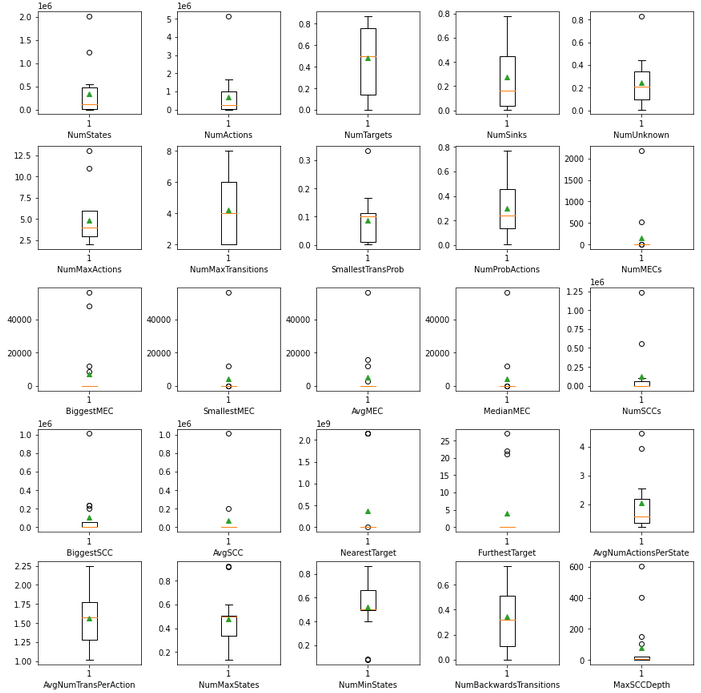
\includegraphics[width=1\textwidth]{figures/Real_FeatureDistribution.png}
    \caption[Feature Distribution of the case studies]{
        Box plot of the feature distribution of the real case studies.
        The orange line marks the median of a feature in all models and the green triangle marks the
        average. The bounds of the boxes mark the 25 and 75 percentile, and the lines extended
        by the whiskers mark the 10 and 90 percentile. Dots outside of whiskers represent
        outliers. For example, the relative number of probabilistic actions is between around
        15\% and 45\% in half of the models. In half of the models, more than 20\% of actions
        are probabilistic.
    }
    \label{fig:Real_FeatureDistribution}
\end{figure}
\FloatBarrier
What we can read from the box plot is this:
\begin{itemize}
    \item According to AvgNumActionsPerState and AvgNumTransPerAction, models have on average 2 actions per state and 1.5 transitions per action
    \item According to NumUnknown, on average 80\% of the states of the models are trivial, and their value can be computed with simple graph algorithms 
    \item Generally, the number of states is evenly split between Maximizer and Minimizer
    \item According to NumProbActions, usually around 70 to 85\% of all actions are deterministic
    \item According to NumMECs, most models do not contain end components
\end{itemize}

By furthermore printing the maximal and minimal occurring values of each feature we obtain that the smallest occurring positive transition probability is 0.001.

With also use the information to draw conclusions about which structural cases do not appear in the real case studies. 
None of the models contain these cases:
\begin{itemize}
    \item Models with numerous actions per state
    \item Models with numerous Transitions per action
    \item Models with very small transition probabilities
\end{itemize}

Furthermore, we use box plots to evaluate for which features our random generation algorithm from Chapter \ref{ch:randomGen} is biased.
Figure \ref{fig:Random_FeatureDistribution} contains the box plots for our randomly generated models.
\begin{figure}[h!]
    \centering
    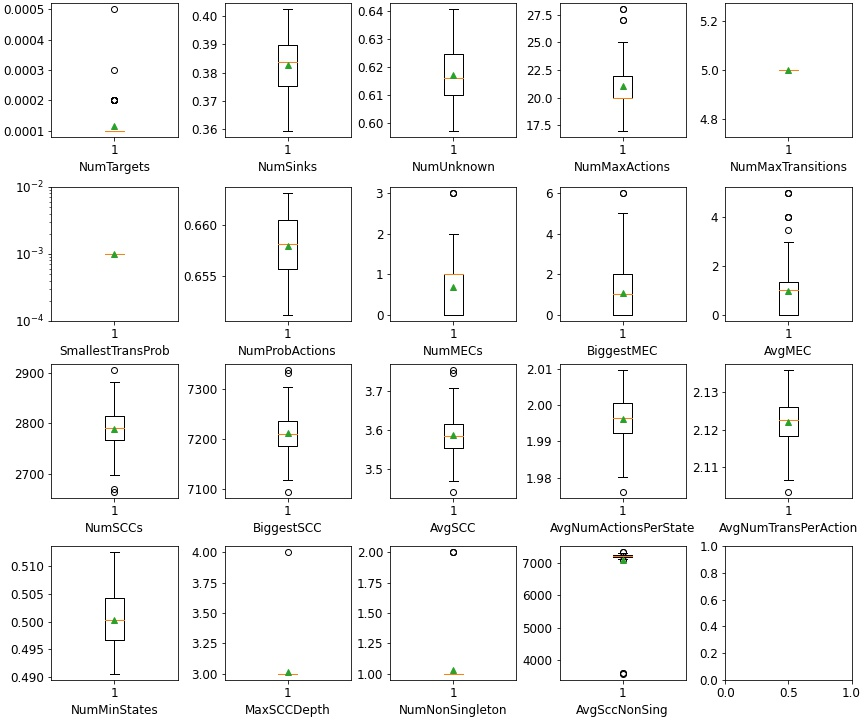
\includegraphics[width=1\textwidth]{figures/RandomRandom_FeatureDistribution.png}
    \caption[Feature Distribution of random models]{
        Feature Distribution of random models
    }
    \label{fig:Random_FeatureDistribution}
\end{figure}
\FloatBarrier

The biases we read from this plot are:
\begin{itemize}
    \item On average, 61.5\% of the states of the models can be computed by trivial graph algorithms. NumSinks shows that almost all known states are sinks.
    \item With the chosen parameters, our algorithm generates models with 2 actions per state on average
     and 2 transitions per action on average.     
     However, our parameters allows us to change the number of actions and transitions per state.
    \item NumNonSingleton shows that in almost all cases there is only one strongly connected component.
        This is because we uniformly randomize where a transition may lead. Thus, it is likely that big SCCs are formed. 
        If necessary, the RandomSCC guideline can control the size of the SCCs.
    \item NumMECs indicates that there is usually either one MEC or none at all. Also, the MECs tend to have very few states (usually no more than 2).
    However, there are parameter configurations such that we form bigger MECs. For example setting the parameters in such a way that the actions are deterministic
    and adding an action to every state in the backwards procedure of Algorithm \ref{alg:randomRandom} creates models with a high tendency of forming few MECs that usually contain the whole state-space.
    Nevertheless, without providing a specific guideline, we have very limited control over the number and size of the MECs.
\end{itemize}

Our random generation algorithm introduces a bias towards various properties like the number of SCCs or the average number of transitions per action. 
To regain control over these properties, we can use other guidelines as described in Section \ref{sec:guidelines}.
\textcolor{red}{Show the Figure of SCC FeatureDistribution for RandomSCC benches.}
However, when comparing the feature distributions of the real case studies and the distributions of the models generated by Algorithm \ref{alg:randomRandom},
they have similar biases for many features. Both benchmarks tend to have few big SCCs, few actions per state, and few transitions per action.
Thus, Algorithm \ref{alg:randomRandom} is capable of recreating models that have in various regards a similar structure to the currently available real case studies. 
\textcolor{purple}{Actually, we might use one box plot for both models}

\section{Algorithm comparison results}

In this section, we compare the Algorithms introduced in Section \ref{sec:SGAlgos} on real case studies, handcrafted examples, and our randomly generated models to both evaluate the 
performance of the algorithms relative to each other and find correlations between model feature values and algorithm performance.

\subsubsection*{Case studies}
We consider case studies from three different sources: 
(i) all real case studies that were already used in~\cite{gandalf}, which are mainly from the PRISM benchmark suite~\cite{PRISMben}.
For a detailed description of the real case studies see Appendix \ref{sec:appendix}
We omit models that are already solved by pre-computations.
(ii) several handcrafted corner case models: haddad-monmege (an adversarial model for value iteration from~\cite{haddadmonmege}), BigMec (a single big MEC), and MulMec (a long chain of many small MECs), the latter two both being from~\cite{gandalf}.
(iii) randomly generated models generated by Algorithm \ref{alg:randomRandom} and our additional guidelines from Subsection \ref{sec:guidelines}.
\textcolor{red}{Here we should state the exact parameters we have used for our models. States are 1000 to 10000, transition probabilities between 0.1 and 0.01 etc.}

First, we provide a general overview of the performance of all algorithms on our benchmarking set in Figure \ref{fig:AlgoPerformance}.
The plots depict the number of solved benchmarks (x-axis) and the time it took to solve them (y-axis). 
For each algorithm, the benchmarks are sorted ascending by verification time. A line stops when no further benchmarks could be solved.
Intuitively, the further to the bottom right a plot is, the better; where going right (solving benchmarks) is more relevant.
The legend on the right is sorted by the performance of the algorithms.
Note that this plot has to be interpreted with care, as it greatly depends on the selection of benchmarks.
\textcolor{purple}{Should make the both plots for real and random in jupyter next to each other. This gives the best quality screenshots. If not possible then at least make the height smaller}
\begin{figure}
    \centering
    \subfloat[\centering Performance Overview on real case studies]{{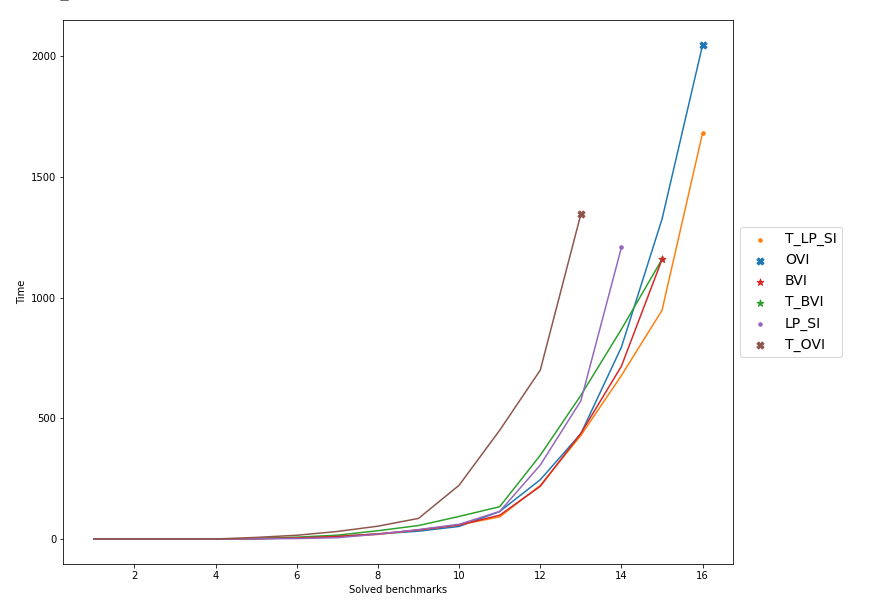
\includegraphics[width=0.8\textwidth]{figures/Real_AlgoPerformance.png} }}%
    \qquad
    \subfloat[\centering Performance Overview on randomly generated models]{{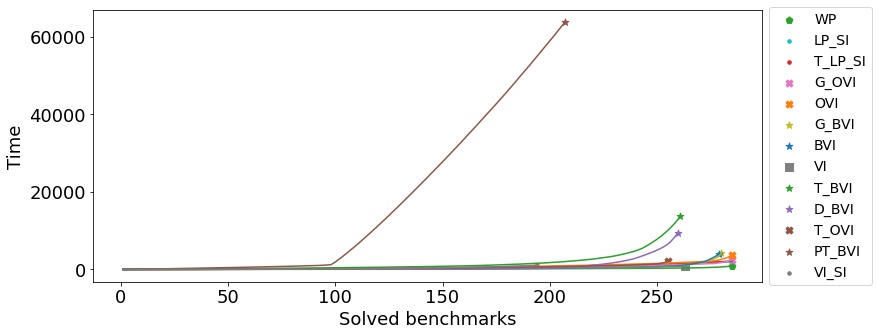
\includegraphics[width=0.8\textwidth]{figures/RandomRandom_AlgoPerformance.png} }}%
    \caption[Overview of Algorithm Performance]{Overview of Algorithm Performance}%
    \label{fig:AlgoPerformance}
\end{figure}

%For value-iteration-based algorithms, we provide the same graph with the number of iterations required to solve the models on the y-axis in Figure
%\ref{fig:AlgoPerformanceIters} \textcolor{red}{Add star-graph for iterations}.

We read several clues from Figure \ref{fig:AlgoPerformance}: 
$\WP$, $\OVI$, and $\TLPSI$ seem to be the most performant algorithms for our benchmarks. 
Also, Optimizations mentioned in Subsection \ref{subsec:optimizations} do not seem to have in general a positive impact on their baseline algorithms.

We split our analysis into three subtopics: 
First, we compare the three value-iteration-based algorithms with guarantees $\OVI$, $\WP$, and $\BVI$. 
Then, we analyze the impact of the optimizations from Subsection \ref{subsec:optimizations} on their respective baseline algorithms.
Lastly, we investigate the performance of $\LPSI$ and $\TLPSI$ in comparison to value-iteration-based algorithms.


\subsection{$\BVI$ vs $\OVI$ vs $\WP$}
We can read from Figure \ref{fig:AlgoPerformance} that WP is the fastest to solve the problems on both random-generated models and real case studies.
To see whether this is the case for all models or only when accumulating runtime, we consider the scatter plot in Figure \ref{fig:WPvsBVIandOVIonRandomRandom}.
Each point in the graph is a model. The x-axis marks the time $\WP$ requires to solve the stochastic game, and the y-axis marks the respective time $\BVI$ or $\OVI$.
The two lines next to the diagonal mark the case that $\WP$ is twice as fast as $\BVI$ / $\OVI$s or half as fast.

\begin{figure}[t]
    \centering
    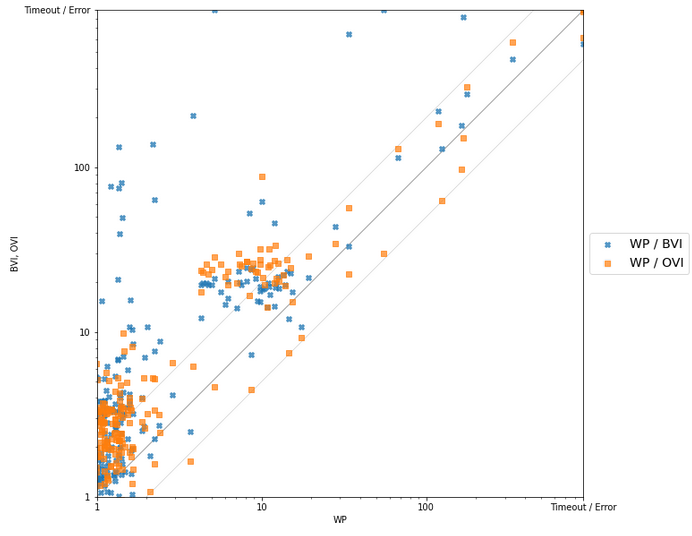
\includegraphics[width=1\textwidth]{figures/WPvsBVIandOVIonAll.png}
    \caption[$\WP$ compared to $\BVI$ and $\OVI$ on time necessary to solve models]{
        $\WP$ compared to $\BVI$ and $\OVI$ on time necessary to solve models
    }
    \label{fig:WPvsBVIandOVIonRandomRandom}
\end{figure}

$\WP$ is usually faster than $\BVI$ and $\OVI$ and never requires more than twice as long.
We are interested in whether there is a correlation between structural properties and $\WP$ being better or worse than the other two.
To inspect the cases where $\WP$ is better than $\OVI$ or the other way around, we plot the feature of the models where one algorithm was at least
1.5 times faster than the other one. Figure \ref{fig:WPvsOVIon1DFeatureScatter} visualizes these cases. 
The red dots mark models where $\OVI$ is at least 1.5 times faster than $\WP$, and the green dots mark models where $\WP$ is at least 1.5 times faster than $\OVI$.
The x-axis displays the range of values that occur for the feature. 
If the dots are clustered for a feature, either one algorithm was only faster if the model had this kind of structural composition, 
or there are only discrete values available for the feature. For example, the number of states is mostly discrete because the random models depend on an input parameter.

\begin{figure}[t]
    \centering
    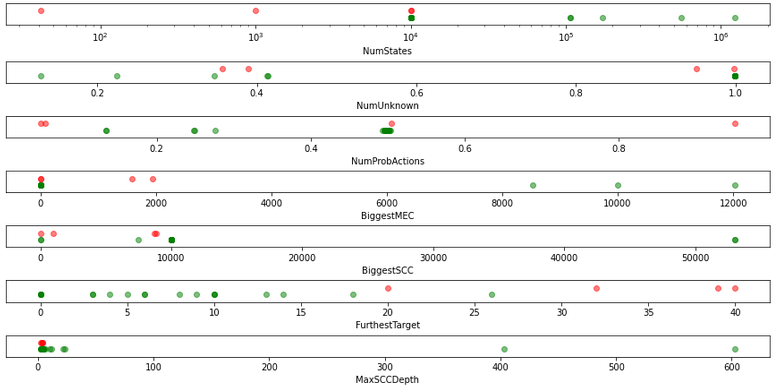
\includegraphics[width=1\textwidth]{figures/WPvsOVIon1DFeatureScatter.png}
    \caption[$\WP$ compared to $\OVI$]{
        The red dots mark models where $\OVI$ is at least 1.5 times faster than $\WP$, and the green dots mark models where $\WP$ is at least 1.5 times faster than $\OVI$.
        The x-axis displays the range of values that occur for the feature. 
        If the dots are clustered for a feature, either one algorithm was only faster if the model had this kind of structural composition, 
        or there are only discrete values available for the feature. For example, the number of states is mostly discrete because the random models depend on an input parameter.
    }
    \label{fig:WPvsOVIon1DFeatureScatter}
\end{figure}

According to Figure \ref{fig:WPvsOVIon1DFeatureScatter}, $\WP$ was better than $\OVI$ if the model had more states, had big MECs and big SCCs.
$\OVI$ seems to be better if the furthest target is far away from the initial state, but since we cannot tie this to any structural significant property,
it may also be noise. If this interpretation is correct, $\WP$ should become even better than $\OVI$ if we use larger models.

The same plot for $\WP$ and $\BVI$ is harder to interpret since there are only two cases where $\BVI$ is 1.5 times faster than $\OVI$, and 40 cases
for the opposite event. Thus, we conclude that $\WP$ is overall more performant on our benchmarks than $\BVI$ regarding runtime. 
\textcolor{blue}{@Maxi: The two cases where BVI is better are quite noisy, so it is not worth including the Figure in my Opinion.
But I have added it in case you think it is interesting. It is Figure \ref{fig:WPvsBVIon1DFeatureScatter}}

\begin{figure}[t]
    \centering
    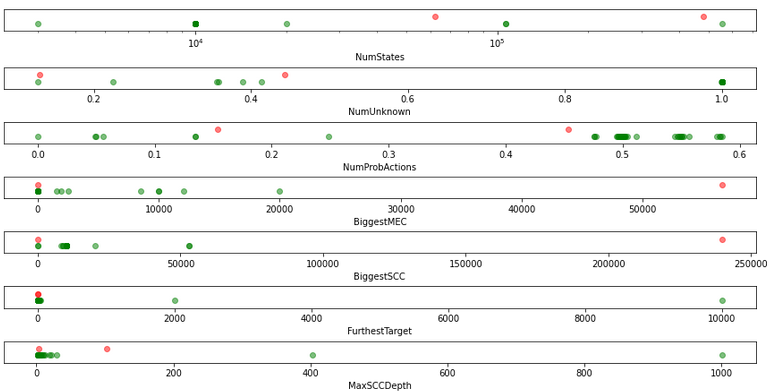
\includegraphics[width=1\textwidth]{figures/WPvsBVIon1DFeatureScatter.png}
    \caption[$\WP$ compared to $\BVI$]{
        Comparing cases where $\WP$ is better than $\BVI$ (green) and $\BVI$ is better than $\WP$ (red) 
        and plotting the corresponding feature values of the models.
    }
    \label{fig:WPvsBVIon1DFeatureScatter}
\end{figure}


However, time is not the best measure we can use to compare value-iteration-based approaches. 
This is because time may be very dependent on optimizations in the code. 
For value-iteration-based algorithms, we can also compare the iteration count, which depends only on the algorithm itself.
Thus, we provide an analogous scatter plot in Figure \textcolor{red}{ITERATION SCATTER} where the axes mark the iterations required to solve a model.

\textcolor{red}{Next, add big models to confirm that the hypothesis you set up also holds for big models. 
There you can also say that although $\OVI$ looks promising in the small models, in the big models it may fall behind $\BVI$ due to unlucky verification phases.}

\subsection{Analyzing the optimizations}

$\mathbf{Gauss-Seidel}$ for $\BVI$:

\textcolor{purple}{Generally fewer iterations, but matrix operations of vanilla is faster than state-by-state.
Can sometimes be worse even for iterations due to unlucky SECs based on lower bound. 
Reversing the order of computation for Gauss-Seidel or using a topological ordering could not improve our results. Show some graphs of how it did not improve}
\textcolor{purple}{Probably, Gauss-Seidel should be even worse for bigger models since there is more room for "not paying off" using state-by-state computation.}


$\mathbf{D}$ for $\BVI$:

\textcolor{purple}{Show time scatter, say two sentences (no huge improvement), go on}

$\mathbf{T}$ for $\BVI, \OVI$ and $\LPSI$:

As the scatter plot \textcolor{red}{Ref to scatter plot TLPSI vs LPSI} shows,
the topological addition for strategy iteration with linear programming in the real case studies and random models does 
neither in- nor decrease the performance of the algorithm considerably.
However, most models have very few SCCs, so the topological optimization does not contribute a lot.
The data point where $\TLPSI$ is significantly faster is on the real case study "dice", where every state is an SCC on its own.
This is obviously the best-case scenario for topological algorithms.
\textcolor{red}{Show Scatter.
Explain why $\OVI$ and $\BVI$ do not scale that well (explained in Gandalf Paper)}

$\TOPAlg$ for $\BVI$:

$\TOPAlg$ seems to perform worse than $\BVI$ in general. This is because we solve the DTMCs with exact methods. 
\textcolor{red}{Scatter BVI vs TOP.}
This requires a matrix inversion, which is an $\mathcal{O}(n^{2})$-operation, where n is the number of states in the SCC whose value is being computed.
The bottleneck becomes apparent if we consider a scatter plot where we show the runtime against the size of the biggest SCC as in Figure \ref{fig:} \textcolor{red}{ADD FEATURE-SCATTER}.
We have also tried solving the resulting MDP with linear programming instead of strategy iteration, but it was still worse than $\TLPSI$.

%There are several relations we read from Figure \ref{fig:AlgoPerformance}:
%\begin{itemize}
%    \item $\TLPSI$ is accumulated better than $\LPSI$.
%    \item $\TLPSI$ is performant for small models
%    \item $\WP$ is usually the best value iteration approach
%    \item $\OVI$ is usually better than $\BVI$ for small models
%    \item $\TOPAlg$ does not seem very promising
%    \item The optimizations do not seem to do much except for the topological switch for $\TLPSI$ and $\WP$
%    \item Why GBVI is not always better than BVI (iterationwise)
%\end{itemize}

\subsection{$\TLPSI$}
\textcolor{red}{It would also be interesting to see if more probabilistic loops affect $\LPSI$ as strong as VI}.

Although value iteration is usually regarded to be the most performant algorithm type for solving stochastic games, 
$\TLPSI$ yielded the best results alongside widest-path bounded value iteration.
Since strategy iteration simply tries to make an informed decision on which strategy to pick and solves the underlying MDP, 
we have to inspect the algorithms we use to solve MDPs - for $\TLPSI$ this is linear programming.

Linear programming scales worse than value iteration for huge models. \textcolor{purple}{To test this, we have 
run several benchmarks on models with state size 10 million and varying SCC sizes. [Now enter Feature-Performance Scatter Plot] 
The bigger the SCCs become, the slower $\TLPSI$ becomes. At a size of [...] per SCC, $\WP$ was faster than $\TLPSI$.}
Thus, we do not recommend using $\TLPSI$ on models with numerous states.
However, $\TLPSI$ may be a good complementary solution approach in case a model is especially hard for value iteration.
Also, the topological improvement allows solving models with huge numbers of small SCCs faster than value iteration.
\textcolor{purple}{And also value iteration was the focus of research for the last 20 years. 
LP could likely be improved. At the moment, we do not even deflate but use MIP to encode the maximum-best-exit constraints. But this should maybe go into future work}


\section{Searching correlations between algorithms and features}
Lastly, we are interested in correlations between algorithm performance and values of features.
Ideally, we would like to find cases where one algorithm scales better with certain features than others.
If we were to find enough such correlations, it would be possible to implement an efficient portfolio solver, which
would analyze the graph structure and decide based on the feature values which algorithm is most likely the best one to use in this case.
To find these correlations, we use the following visualization tools:

\textcolor{purple}{I am not really sure what I want to do with this section. 
But it would be a cool place to show algorithm-feature correlations and to show the ideas we applied to search for correlations.
Maybe I should instead make a separate section with all graph types that is easy to look up.}

\textcolor{red}{Maybe search for some scatters where the algorithms differ a lot and show them.}

\subparagraph*{Heatmaps}
Heatmaps visualize correlation matrices - matrices where one feature is mapped against another. The higher the correlation value, the stronger
a correlation between two features is. On the diagonal of the matrix, the correlation is maximal since there is a directly proportional correlation between
a feature and itself. Ideally, we would like to get clues from the heatmap which features or correlations we should investigate.
However, for the most part, we could not gather any non-trivial information from heatmaps. \textcolor{purple}{This is also tricky because
there is only one type of correlation that can be shown effectively: Most often we search for linear correlation with heatmaps. Thus,
if one feature depends in a non-linear fashion on another - for example if it rises quadratically - the correlation value may still be very low.}

\subparagraph*{Feature-performace scatter plots}
We plot algorithm runtime / iterations against feature values.

What is there to find in these graphs?
\begin{itemize}
    \item Clearly visible how TOP scales with SCC-size
    \item All scale with number of unknowns, which is no surprise but might be mentioned.
\end{itemize}

\subparagraph*{One dimensional scatter plots for features}
We can define two events A, B. Then we get models where A happens, models where B happens and then plot the feature values for models that are in set A or set B.
This way, we can find clusters and make conclusions like "If A happens, then the models have these feature values."
\chapterSpace
\chapter{Conclusion and future work} \label{ch:conclusion}
In this thesis we introduced a toolset to randomly generate models to enrich the structural variety of available models.
This enabled a broader and more precise comparison of the available solution algorithms.

Our randomly generated models can be in adjusted in a way that resembles the currently available case studies we are aware of.
At the same time, we are able to adjust the parameters and guidelines in such a way that they do express structural properties that differ from the case studies.
The only limit we face at the moment is that explicit models can be parsed only slowly in PRISM. 
To avoid this issue, we provide the option to prepend graphs at runtime.

Furthermore, we explored were helpful to analyze the growing set of both models and algorithms to analyze.
Establishing analysis tools allowed us to prototype algorithm ideas, assess fast whether it seems promising,
and provide a better overview of the data we collect. 
Lastly, our tools for model analysis improve with increasing data points.
This is not the case for tables as visualization and analysis tool, 
but they are nevertheless frequently the only utility used for visualization in analysis \cite{paperMaxi}\cite{widestPath}\cite{learningBased}.

Lastly, we have compared algorithms for $\SG$ solving and have found that although $\TLPSI$ is not competitive to $\OVI$, $\BVI$ and $\WP$ for large models,
it may be a good alternative for games that are adversarial to approached based on value iteration. 
Furthermore, it may be a good approach in case a model has many SCCs that are all of small size.

Like $\TLPSI$, $\OVI$ seemed promising for smaller models, but could not keep up with $\WP$ and $\BVI$ for large models.
Thus, for now we conclude in general one should try $\BVI$ or $\WP$ when trying to solve a stochastic reachability game, 
and should pivot to other methods if these approaches struggle to converge.

\section*{Future work}
The model features we analyze at the moment helped us to draw some conclusions, but there are still many questions unanswered that would require
additional structural concepts and features that we track.
These questions are for example when to use Gauss-Seidel optimization or when to use $\WP$ instead of $\BVI$.

In addition, there are still many data analysis techniques we did not implement yet like stochastic tests or artificial intelligence algorithms
that can cluster features and find correlations between them. 

We believe more research of the correlation between algorithm performance and structural properties gives way to a portfolio solver which could first
analyze important structural features and then pick heuristically the most adapt algorithm to solve the problem.
With enough models, the decision which algorithm to use may be made by a neural network.
Also, combinations of algorithms like $\OVI$ and $\BVI$ could then be used effectively in a fitting scenario.
The user would have to pay the overhead for computing more vectors but may converge faster.

Since algorithm performance may change drastically depending on the models size,
we need to resolve the issue that our random generation process creates large explicit files which PRISM cannot handle.
The next step would be to create an optimization system to our random generation algorithm that would hold chunks of the data in 
implicit blocks to make the files easier parsable.

Lastly, at the moment, our random generation algorithm enforces a tendency of states with smaller indices to have more actions than states with higher indices.
Ideally, the user should be able to remove this restriction.
This could be addressed by introducing mechanisms like for example that a state $\stateMac_i$ can only be connected to states $\stateMac_{j}$ with $j \in [i-50, i+50]$.
%\input{3_qp/qp_main}
%\chapterSpace
%\chapter{Conclusion and future work} \label{ch:conclusion}
In this thesis we introduced a toolset to randomly generate models to enrich the structural variety of available models.
This enabled a broader and more precise comparison of the available solution algorithms.

Our randomly generated models can be in adjusted in a way that resembles the currently available case studies we are aware of.
At the same time, we are able to adjust the parameters and guidelines in such a way that they do express structural properties that differ from the case studies.
The only limit we face at the moment is that explicit models can be parsed only slowly in PRISM. 
To avoid this issue, we provide the option to prepend graphs at runtime.

Furthermore, we explored were helpful to analyze the growing set of both models and algorithms to analyze.
Establishing analysis tools allowed us to prototype algorithm ideas, assess fast whether it seems promising,
and provide a better overview of the data we collect. 
Lastly, our tools for model analysis improve with increasing data points.
This is not the case for tables as visualization and analysis tool, 
but they are nevertheless frequently the only utility used for visualization in analysis \cite{paperMaxi}\cite{widestPath}\cite{learningBased}.

Lastly, we have compared algorithms for $\SG$ solving and have found that although $\TLPSI$ is not competitive to $\OVI$, $\BVI$ and $\WP$ for large models,
it may be a good alternative for games that are adversarial to approached based on value iteration. 
Furthermore, it may be a good approach in case a model has many SCCs that are all of small size.

Like $\TLPSI$, $\OVI$ seemed promising for smaller models, but could not keep up with $\WP$ and $\BVI$ for large models.
Thus, for now we conclude in general one should try $\BVI$ or $\WP$ when trying to solve a stochastic reachability game, 
and should pivot to other methods if these approaches struggle to converge.

\section*{Future work}
The model features we analyze at the moment helped us to draw some conclusions, but there are still many questions unanswered that would require
additional structural concepts and features that we track.
These questions are for example when to use Gauss-Seidel optimization or when to use $\WP$ instead of $\BVI$.

In addition, there are still many data analysis techniques we did not implement yet like stochastic tests or artificial intelligence algorithms
that can cluster features and find correlations between them. 

We believe more research of the correlation between algorithm performance and structural properties gives way to a portfolio solver which could first
analyze important structural features and then pick heuristically the most adapt algorithm to solve the problem.
With enough models, the decision which algorithm to use may be made by a neural network.
Also, combinations of algorithms like $\OVI$ and $\BVI$ could then be used effectively in a fitting scenario.
The user would have to pay the overhead for computing more vectors but may converge faster.

Since algorithm performance may change drastically depending on the models size,
we need to resolve the issue that our random generation process creates large explicit files which PRISM cannot handle.
The next step would be to create an optimization system to our random generation algorithm that would hold chunks of the data in 
implicit blocks to make the files easier parsable.

Lastly, at the moment, our random generation algorithm enforces a tendency of states with smaller indices to have more actions than states with higher indices.
Ideally, the user should be able to remove this restriction.
This could be addressed by introducing mechanisms like for example that a state $\stateMac_i$ can only be connected to states $\stateMac_{j}$ with $j \in [i-50, i+50]$.

\microtypesetup{protrusion=false}
\listoffigures{}
%\listoftables{}
\microtypesetup{protrusion=true}
\printglossaries
\printbibliography{}

\appendix{}
\chapter{Appendix: Information about the models} \label{sec:appendix}

\section*{Random model generation parameters} \label{sec:GenParams}
In this section we present the parameters we have used to generate the 300 randomly generated models. 
We have generated three sets of random models: Two for Algorithm \ref{alg:randomRandom} referred to as RandomA and RandomB with a distinct set of parameters, and one with the RandomSCC guideline.
While we have also tried and used the RandomTree guideline, we did not include it in our benchmarks due to a lack of time.
All randomly generated models can be found in the GitHub Repository \url{https://github.com/ga67vib/Algorithms-For-Stochastic-Games} in the folder \texttt{random-generated-models}.
The difference between the RandomA and RandomB is that in one every state has 10 actions,
and in the other one we decided for a lower number of actions. The feature distributions of RandomA are displayed in Figure \ref{fig:Random_FeatureDistribution}, 
and the feature distribution of the set created with the RandomSCC guideline are displayed in Figure \ref{fig:RandomSCC_FeatureDistributions}.
The parameters we have used to generate these models were the following:
\begin{center}
	\begin{tabular}{| c | c c c |} 
	 \hline
	 Parameter & RandomA & RandomB & RandomSCC \\ [0.5ex] 
	 \hline\hline
	 size & 10000 & 10000 & 10000 \\
	 \hline
	 numModels & 100 & 100 & 100 \\
	 \hline
	 guideline & - & - & RandomSCC \\
	 \hline
	 smallestProb & $10^{-2}$ & $10^{-3}$ & $10^{-3}$ \\
	 \hline
	 backwardsProb & 1 & 1 & 1 \\ [1ex] 
	 \hline
	 maxBranchNum & 10 & 10 & 10 \\ [1ex] 
	 \hline
	 forceUnknown & false & false & true \\ [1ex] 
	 \hline
	 branchingProb & 1 & 0.75 & 0.75 \\ [1ex] 
	 \hline
	 maximizerProb & 0.5 & 0.5 & 0.7 \\ [1ex] 
	 \hline
	 minIncomingActions & 2 & 10 & 10 \\ [1ex] 
	 \hline
	 maxIncomingActions & 4 & 12 & 12 \\ [1ex] 
	 \hline
	 maxBackwardsActions & 1 & 1 & 10 \\ [1ex] 
	 \hline
	 minSCCSize & - & - & 1000 \\ [1ex] 
	 \hline
	 maxSCCSize & - & - & 2000 \\ [1ex] 
	 \hline
	\end{tabular}
\end{center}
	

%\section{More Formal Random Generation Algorithm}
%
%
%\textcolor{purple}{Basically, replace every function Im speaking about with a tuple (which it formally is) and do set-operations. 
%Not as nice in my opinion as a descriptive approach. This is not done yet. Also I will need a formal fill actions.
%Whenever you add an action with a transition distribution that sums up to one, every state NOT reached must be added with transition probability 0.}
%\begin{algorithm}[ht]
%  \label{alg:randomRandomFormal}
%  \caption{Generating random models connected from initial state}
%  \begin{algorithmic}[1]
%  \Ensure Stochastic game $\SG$ where the initial state is connected to any $\state \in \states$
%  \State Create $\states$ with a random $n \in \Naturals$
%  \State Partition $\states$ uniformly at random into $\maxStates$ and $\minStates$
%  \State Enumerate $\state \in \states$ in any random order from 0 to n-1
%  \State Set $\initstate$ to the state with index 0
%  \State $\trans = \emptyset$
%  \State $\actions = \emptyset$
%  \For{$\state = 0 \rightarrow n-1$} $\Av(\state) = \emptyset$\EndFor
%  \For{$\state = 1 \rightarrow n-1$} \Comment{Forward Procedure}
%      \If{$\exists \state' \in \states, \action \in \actions: \trans(\state', \action, \state) > 0$} 
%          Skip state
%      \Else
%          \State Pick any state $\state'$ with index smaller than $\state$
%          \State Pick a random $p \in (0, 1]$
%          \State Create a new action $\action$
%          \State $\actions \gets \actions \union \{action\}$
%          \State $\trans \gets \trans \union \{(\state', \action, \state, p)\}$
%          \State Make $\action$ a valid action by applying FillAction($\state'$, $\action$)
%          \State $\Av(\state') \gets \Av(\state') \union \{action\}$
%      \EndIf
%  \EndFor
%  \For{$\state = n - 1 \rightarrow 0$} \Comment{Backward Procedure}
%      \State Pick a random number $m \in [M - |\Av(\state)]$ \Comment{Add as many actions as possible}
%      \If{$|\Av(\state)| = 0$} $m \gets \max{\{m, 1\}}$ \Comment{Every state needs to have at least one action} \EndIf 
%      \For{$i = 1 \rightarrow m$}
%          \State $(\state, \action<i>)$ = FillAction($\state$, $\action<i>$)
%          \State Add $\action<i>$ to $\Av(\state)$
%          \State Add $\action$ to $\actions$
%      \EndFor
%  \EndFor
%  \end{algorithmic}
%\end{algorithm}
%


\end{document}
